\documentclass{article}

\usepackage{parskip}
\usepackage{amsmath}
\usepackage{amssymb}
\usepackage{graphicx}
\usepackage{xltabular}
\usepackage{xcolor}
\usepackage{eurosym}

\usepackage[style=apa]{biblatex}
\addbibresource{references.bib}

\usepackage{setspace}
\onehalfspacing

\usepackage{geometry}
\geometry{
    top=3cm,
    bottom=3cm,
    left=2.5cm,
    right=2.5cm
}

\usepackage{fancyhdr}
\fancypagestyle{fancy}{
    \fancyhf{}
    \renewcommand{\headrulewidth}{0.8pt}
    \fancyhead[L]{\textit{\leftmark}}
    \fancyfoot[C]{\thepage}
}
\renewcommand{\sectionmark}[1]{\markboth{\thesection. #1}{}}
\newcommand{\setupappendixheaders}{%
    \renewcommand{\subsectionmark}[1]{\markboth{Appendix \thesubsection: ##1}{}}%
}
\renewcommand{\contentsname}{Contents}
\pagestyle{fancy}

\usepackage{chngcntr}
\AtBeginDocument{
  \counterwithin{figure}{section}
  \counterwithin{table}{section}
}

\usepackage{hyperref}
\hypersetup{
    colorlinks=true,
    citecolor=black,
    filecolor=black,
    linkcolor=black,
    urlcolor=black
}
\usepackage{caption}
\newcommand{\autorefapdx}[1]{\hyperref[#1]{appendix~\ref*{#1}}}

\usepackage{tikz}
\tikzstyle{node:input}=[circle,draw,minimum size=1.28cm,fill=green!20]
\tikzstyle{node:inputlabelcolor}=[green!60!black]
\tikzstyle{node:hidden}=[circle,draw,minimum size=1.28cm,fill=blue!20]
\tikzstyle{node:hiddenlabelcolor}=[blue!60!black]
\tikzstyle{node:output}=[circle,draw,minimum size=1.28cm,fill=red!20]
\tikzstyle{node:outputlabelcolor}=[red!60!black]
\tikzstyle{node:gate}=[circle,draw,minimum size=1.28cm,fill=yellow!30]
\tikzstyle{node:gatelabelcolor}=[yellow!70!black]
\tikzstyle{node:operation}=[circle,draw,minimum size=1cm,fill=gray!20]
\tikzstyle{draw:connection}=[-latex, thick, rounded corners=4pt]

\newcommand{\cotwo}{CO$_{2}$}
\newcommand{\cotwoe}{CO$_{2}$e}

\renewcommand{\arraystretch}{1.3} % sets tables to extra 30% space vertically

\begin{document}

\thispagestyle{empty}

\begin{titlepage}
    \thispagestyle{empty}

    \begin{center}
        {\Large \textbf{Aarhus University}}

        Department of Economics and Business Economics

        \vspace{1cm}

        {\large Master's Thesis}

        {\large June 2025\par}

        \vspace{0.8cm}

        \rule{\linewidth}{1pt}\par

        \vspace{0.5cm}

        {\huge \textbf{Short-Term Carbon Emission Forecasting in Volatile Wind Power Grids using LSTM Neural Networks}}

        \vspace{0.15cm}
        \rule{\linewidth}{1pt}\par

        \vspace{1cm}

        {\large Martin Bøge Jørgensen (202007452)}

        Supervisor: Associate Professor Allan Würtz

        \vfill

        \includegraphics[width=8cm]{sections/figures/au_bss_logo.eps}

        \vspace{0.5cm}

        Character count (including blanks; each table and figure as 800 chars): \input{.char_count.main.txt}/ 132,000 (limit).
        \normalsize
    \end{center}
\end{titlepage}


\thispagestyle{plain}

Master's thesis written by Martin Bøge Jørgensen\\
Business Intelligence (cand.merc)\\
School of Business and Social Sciences\\
Aarhus University\\

\vfill

Copyright \copyright \space Martin Bøge Jørgensen, June 2025. This thesis is licensed under the \href{https://creativecommons.org/licenses/by-nd/4.0/}{Creative Commons Attribution-NoDerivatives 4.0 International License (CC BY-ND 4.0)}.

The full source code for this thesis is available in the public repository: \href{https://github.com/MartinBoge/masters-thesis}{\texttt{github.com/MartinBoge/masters-thesis}}.

The accompanying code located in the \texttt{analysis/} directory is licensed under the \href{https://opensource.org/licenses/MIT}{MIT License}.


%COUNT:abstract
\thispagestyle{plain}
\section*{Abstract}
\addcontentsline{toc}{section}{Abstract}

Rising carbon emissions and the global transition to renewable energy have created an urgent need for accurate short-term carbon emission forecasting in volatile wind power grids. Denmark's western bidding zone (DK1), with over 50\% wind generation, exemplifies the forecasting challenges faced by modern renewable-dominated power systems. The volatile wind generation patterns, coupled with market-based balancing mechanisms and cross-border electricity flows, result in carbon emission dynamics characterized by nonlinear relationships and complex temporal dependencies that traditional statistical approaches struggle to capture effectively. This thesis addresses the fundamental question of how long short-term memory neural networks can be designed for short-term (1-24 hour) carbon emission forecasting in DK1 to improve prediction accuracy compared to simple benchmark models and traditional autoregressive approaches.

This thesis develops and evaluates two LSTM architectures using three years of hourly data (2022-2025) encompassing carbon emissions and explanatory variables including renewable generation forecasts, consumption patterns, market prices, and meteorological conditions. The methodology employs a single-layer LSTM for 1-hour ahead forecasting and an encoder-decoder architecture for 24-hour ahead prediction, with systematic hyperparameter optimization conducted through coordinate descent. Performance is evaluated against naive persistence and optimally-configured ARIMA baselines using statistical significance testing via Diebold-Mariano tests.

The results demonstrate substantial forecasting improvements across both prediction horizons. For 24-hour ahead prediction, the encoder-decoder LSTM achieves an 11.3\% reduction in RMSE compared to ARIMA models and a 25.4\% reduction compared to naive persistence, with all improvements confirmed as statistically significant. Feature importance analysis reveals that forecasted solar photovoltaic production emerges as the most influential exogenous predictor despite the dominance of wind-power in DK1. This interestingly reveals that renewable power sources with more predictable generation patterns provide a better signal compared to those of larger share of the total renewable generation mix.

The practical implications extend beyond academic interest to tangible economic and environmental benefits. Conservative estimates indicate that a medium-sized manufacturing company could achieve annual carbon reductions of 855 to 1,905 tonnes \cotwoe{} through optimized production scheduling enabled by accurate emission forecasts, representing cost savings of \euro72,700 to \euro161,900 at current carbon prices. For transmission system operators, enhanced forecasting enables proactive grid management strategies that could reduce emergency reserve activations, yielding operational savings of \euro3.2 to \euro7.1 million annually while avoiding 8,500 to 19,000 tonnes \cotwoe{} in emissions.

This thesis establishes LSTM neural networks as an effective solution for carbon emission forecasting in wind-dominated grids, addressing a significant research gap in renewable energy forecasting. The demonstrated accuracy improvements and quantified economic benefits provide compelling justification for deploying advanced forecasting architectures in industrial demand response systems and grid operations. As electricity systems worldwide pursue aggressive renewable integration targets similar to DK1's profile, the forecasting methodologies developed offer a deeper understanding of carbon emission forecasting in wind-dominated grids while supporting both economic efficiency and climate objectives in the transition to sustainable power generation.

%COUNT:endabstract

\thispagestyle{plain}
\section*{Acknowledgements}
\addcontentsline{toc}{section}{Acknowledgements}

A special thanks to \href{https://www.energyquantified.com/}{Energy Quantified} for generously providing access to their power market data, essential for this thesis.


\thispagestyle{plain}
\setcounter{tocdepth}{2}
\tableofcontents
\markboth{Contents}{}


%COUNT:main
\thispagestyle{plain}
\section{Introduction}

Rising carbon emissions are destabilizing our climate system, causing global temperature increases, extreme weather events, and threatening ecosystems worldwide. A rapid and comprehensive transition to green energy sources is therefore essential to prevent further environmental degradation and secure a sustainable future for coming generations. To effectively manage the transition to green energy systems an element is the ability to accurately forecast short-term carbon emissions. These forecasts function as a practical tool in production planning for manufacturing companies and in grid management for a Transmission System Operator (TSO).

Manufacturing companies, particularly in energy-intensive sectors, are increasingly focusing on reducing their carbon footprints and complying with stringent emission regulations. By aligning energy-intensive processes with periods of lower carbon emissions, manufacturers can reduce their carbon footprint. For example, AI-driven scheduling can shift high-energy tasks to times when the electricity grid is greener, thereby enhancing sustainability \parencite{futurebridge}.

In the energy sector, a TSO is an organization responsible for operating, maintaining, and developing the grid supplying electricity and natural gas in a particular region or country. The \citeauthor{entsoe2022} (ENTSO-E) emphasizes the necessity for enhanced system flexibility and advanced operational strategies to manage the increasing integration of renewable energy sources. In their vision for a carbon-neutral Europe, ENTSO-E highlights that the future power system will be highly weather-dependent, necessitating significant flexibility to maintain system adequacy and resilience. This underscores the critical role of accurate short-term carbon emissions forecasts in enabling TSOs to balance supply and demand effectively \parencite{entsoe2022}.

Considering this challenge, especially in weather-dependent power grids, an intriguing case is Denmark's western bidding zone (DK1). In DK1 wind power generation accounts for over 50 percent of its electricity mix \parencite{wang2017,iea2023}, one of the highest shares worldwide. Moreover, many power systems are setting similar ambitious targets with for instance Germany that aims to reach 80 percent renewable electricity by 2030 and 100 percent by 2035, with wind power playing a major role \parencite{iea2025}. The unique characteristics of DK1 make it an ideal setting for studying the relationship between renewable energy variability and carbon emissions. Unlike more hydropower-dominated grids, where storage capacity can smooth out fluctuations, DK1 further relies on market-based mechanisms, cross-border electricity trading, and flexible generation to maintain system stability \parencite{energistyrelsen}.

\subsection{Research Context}

The operational characteristics of DK1 with a high share of renewable energy sources create significant forecasting challenges that extend beyond traditional time series modeling capabilities. The volatile wind generation patterns, coupled with market-based balancing mechanisms and cross-border electricity flows, result in carbon emission dynamics characterized by nonlinear relationships, regime changes, and complex temporal dependencies that span multiple time scales \parencite{carlini2023}. Traditional statistical approaches such as autoregressive models, while valuable for their interpretability, are fundamentally limited in their ability to capture these intricate patterns and sudden shifts in generation mix composition \parencite{box2015, hyndman2021}.

Machine learning approaches designed for sequential data offer promising alternatives for addressing these modeling challenges. Long short-term memory neural networks (LSTM) have demonstrated particular effectiveness in energy forecasting applications due to their ability to selectively retain relevant information across different time horizons while adapting to new conditions \parencite{hochreiter1997}. The gating mechanisms of LSTMs enable it to maintain context about weather patterns, generation schedules, and market dynamics for appropriate durations, making it well-suited for the temporal complexity inherent in wind-dominated systems \parencite{ostermann2024,pierre2023}.

However, the existing literature reveals a significant research gap regarding LSTM applications in highly renewable-integrated bidding zones. Most carbon emission forecasting studies focus on larger national grids or systems with different renewable profiles, while the specific challenges of wind-dominated zones like DK1 remain largely unexplored \parencite{ostermann2024, bokde2021}. This gap is particularly significant given that DK1's operational characteristics are increasingly representative of future power systems as countries pursue aggressive renewable energy targets. Understanding how advanced neural network architectures perform in this challenging environment provides crucial insights for the growing number of power systems following similar renewable integration pathways.

\subsection{Problem Statement}

\newcommand{\researchquestion}{
    \begin{quote}
        \textit{How can long short-term memory neural networks be designed for short-term (1--24 hour) \cotwo{} emission forecasting in Denmark's wind-dominated DK1 bidding zone to improve prediction accuracy compared to simple benchmark models and traditional autoregressive models?}
    \end{quote}
}

Given the identified research gap and the critical operational needs of renewable-heavy power systems, this thesis addresses a fundamental challenge in modern grid management. The intersection of high wind penetration, volatile generation patterns, and complex market dynamics in DK1 creates carbon emission forecasting challenges that existing methodologies struggle to address effectively. While traditional statistical approaches remain valuable for their interpretability, their fundamental limitations in capturing nonlinear relationships and regime changes necessitate exploration of more sophisticated modeling approaches capable of handling the temporal complexity inherent in wind-dominated systems.

The main research question for this thesis becomes: \researchquestion{}

This question encompasses several critical dimensions that define the scope and approach of this thesis. The focus on "\textit{long short-term memory neural networks}" reflects the need for architectures capable of learning complex temporal dependencies and adapting to the dynamic operational conditions characteristic of renewable-heavy grids. The phrase "\textit{designed for}" emphasizes that this is not merely an application of existing LSTM models, but rather a systematic exploration of architectural configurations, hyperparameters, and design choices optimized specifically for carbon emission patterns in volatile wind systems. The "\textit{short-term (1--24 hour)}" specification addresses practical operational requirements, spanning from immediate decision-making support to day-ahead planning horizons essential for grid management and industrial scheduling. The geographic focus on "\textit{Denmark's wind-dominated DK1 bidding zone}" provides a strategically valuable case study whose operational characteristics are increasingly representative of future power systems worldwide. Finally, the commitment to "\textit{improve prediction accuracy compared to simple benchmark models and traditional autoregressive models}" establishes a rigorous evaluation framework that demands demonstrable performance gains over both naive approaches and established statistical methods.

The sub questions to help guide this thesis becomes:

\begin{enumerate}
    \item What architectural configurations and hyperparameters optimize LSTM performance for capturing carbon emission patterns in the DK1 zone?
    \item Which input features and feature engineering strategies most significantly enhance LSTM predictive performance for short-term carbon emissions forecasting?
    \item How does the forecasting horizon (1-hour vs 24-hour ahead) affect model performance and required architectural adaptations?
    \item What quantifiable improvements in prediction accuracy can LSTM models achieve compared to benchmark models and traditional autoregressive approaches for the DK1 zone?
    \item To what extent could manufacturing companies operating in DK1 and Energinet realize economic and carbon reduction benefits from enhanced carbon emission forecasting accuracy?
\end{enumerate}

These sub questions provide a systematic framework for addressing the main research question through technical, empirical, and practical dimensions. The first three sub questions guide the technical development: exploring LSTM design choices specific to carbon emission dynamics, directing attention toward optimal feature engineering strategies, and enabling systematic comparison across different forecasting horizons to reveal how model requirements evolve with prediction complexity. The fourth sub question establishes the empirical validation framework necessary to demonstrate quantifiable improvements relative to existing forecasting methods. The fifth sub question extends beyond technical performance to evaluate the practical economic and environmental benefits for key stakeholders in the DK1 system. Together, these sub questions structure the thesis to provide theoretical insights into LSTM capabilities, empirical validation of performance gains, and practical guidance for implementing advanced forecasting systems that deliver measurable value in renewable-heavy power grids.

\subsection{Thesis Structure}

This thesis is structured to systematically address the research question through a logical progression from theoretical foundations to empirical findings. Following this introduction, the literature review examines existing approaches to short-term carbon emission forecasting and energy prediction, identifying methodological insights and establishing the research gap that motivates this DK1-focused investigation. The theory section provides the mathematical and architectural foundations necessary for understanding neural networks and LSTM architectures, progressing from basic feed-forward networks through recurrent architectures to the specialized gating mechanisms that enable LSTMs to capture long-term temporal dependencies. The methodology section details the systematic approach employed for model development, including data collection and preprocessing procedures, LSTM architectural design choices, baseline model establishment, and evaluation frameworks for both a 1-hour and 24-hour forecasting horizon. The results section presents comprehensive empirical findings, encompassing baseline model performance, LSTM hyperparameter optimization outcomes, forecasting accuracy comparisons, and feature importance analysis that validates the theoretical foundations underlying the variable selection. The discussion synthesizes these findings to address the research question and sub questions, evaluating the practical implications for renewable energy forecasting while identifying limitations and directions for future research. Finally, the conclusion provides a concise summary of key findings, contributions to the field, and recommendations for future work in carbon emission forecasting for renewable energy systems.


\thispagestyle{plain}
\section{Literature Review}
\label{sec:lit}

This section examines the academic literature on short-term (hourly and up to 24-hour ahead) carbon emissions forecasting, with a focus on the applied methodologies. Furthermore, it covers relevant discussions and findings related to the research question and related work within short-term energy forecasting (e.g. load and wind forecasting), since the techniques often carry over to predicting carbon emissions. Key questions addressed include: (1) What are the typical methodologies used for short-term carbon emissions forecasting or similar energy forecasts? (2) What methodological and practical insights from past studies are relevant for this thesis? (3) Why is DK1 an interesting and unique case compared to other regions? and (4) What research gap can be identified for a DK1-focused study? This literature review establishes the methodological foundation for this thesis while highlighting the research gap in carbon emissions forecasting for the DK1 region that this work aims to fill.

\subsection{Modeling Approaches in Short-Term Emissions and Energy Forecasting}

The methodologies in short-term forecasting methods span a spectrum from classical statistical techniques like autoregressive integrated moving average (ARIMA) \parencite{box2015}, exponential smoothing (e.g. Holt-Winters) \parencite{hyndman2021}, state-space/Kalman filter models \parencite{durbin2001} and structural decomposition \parencite{harvey1993} to more flexible machine-learning approaches such as linear regression \parencite{douglas2021} and nonlinear regression \parencite{seber2003}, random forests \parencite{breiman2001}, gradient-boosted trees (e.g. XGBoost) \parencite{chen2016} and support-vector regression \parencite{drucker1997}, and finally to deep-learning architectures tailored for sequential data, including recurrent neural networks (RNNs) \parencite{elman1990}, long short-term memory neural networks (LSTMs) \parencite{hochreiter1997} and gated recurrent unit models (GRUs) \parencite{cho2014}, temporal convolutional networks (TCNs) \parencite{bai2018} and Transformer-based encoders/decoders \parencite{vaswani2017}. Hybrid and ensemble schemes that blend statistical and learning-based models have also proven effective \parencite{zhang2003}.

In the literature there is a handful of studies that directly forecast carbon emissions or intensity. Expanding the scope to energy related forecasts there are even more to draw meaningful insights from. A closely related study to the forecasting problem in this thesis is \citetitle{ostermann2024} by \textcite{ostermann2024}, which forecasts the hourly carbon intensity of Germany's electricity mix up to 24 hours ahead. It applies a SARIMAX (seasonal ARIMA with exogenous variables) model as a representative traditional approach, and compares it with various machine learning models (bagging, random forests, gradient boosting) and deep learning models (CNN, LSTM, MLP) using 2019-2022 data. All the advanced models outperformed baseline persistence forecasts, for example, gradient boosting achieved the lowest mean absolute percentage error. The SARIMAX model performed respectably but was less accurate than the best non-parametric (ML) models. Notably, the authors observe that their deep learning models did not fully outperform simpler methods, cautioning that the added complexity of deep learning must be justified by significant accuracy gains. They suggest weighing implementation effort against incremental benefit when considering complex models in practice.

Another great example is the study \citetitle{bokde2021} by \textcite{bokde2021}. This study proposes a time-series decomposition method to forecast electricity-related \cotwo{} emissions on a short-term basis (up to 48 hours, aligning with the day-ahead market). The approach breaks the emissions time series into components (e.g. trend, seasonal, residual) and forecasts each component with appropriate models (statistical or machine learning), then recombines them. In performance benchmarks on national data, the proposed method delivered significantly improved accuracy - for instance, in France it achieved a MAPE about 25\% lower than the best existing state-of-the-art model. The authors demonstrate the method across five European countries (France, Germany, Norway, Denmark, Poland) and show that smart scheduling using these forecasts can substantially cut emissions (e.g. the 25\% reduction in France by shifting a 4-hour load block to greener periods). While the focus was on enhancing classical forecasting via decomposition, it implicitly compares against other models (some of which include machine learning), showing the decomposition strategy can rival or beat more complex approaches. However, they do not explore the use of deep learning.

Given this thesis focuses on DK1, the study by \textcite{leerbeck2020} is particularly relevant. This study forecasts hourly average and marginal \cotwo{} emission factors for the DK2 region (Eastern Denmark) with a 1--24 hour horizon. The methodology begins with a large set of 473 candidate features (including grid production, demand, weather from Denmark and neighbors) which is then pruned to \textless30 via LASSO and forward selection. The forecasting model itself combines three specialized linear regression models (to capture different nonlinear effects) into an ensemble, and then applies an ARIMA model to the residuals of the ensemble - effectively yielding an ARIMAX (ARIMA with exogenous inputs) , i.e., they construct a hybrid model. This traditional-meets-ML approach proved useful. The normalized RMSE ranged from 0.095 to 0.183 for average emission intensity and 0.029 to 0.160 for marginal intensity (1-hour ahead being most accurate). The model also produced well-calibrated prediction intervals, addressing the uncertainty in \cotwo{} forecasts. The authors note that marginal emissions in DK2 appeared uncorrelated with local features (suggesting marginal generators are often outside the zone), an insight gained from the linear model coefficients. They do not explicitly compare against deep learning, but the study demonstrates that a carefully constructed linear/ARIMA hybrid (with feature engineering) can achieve high accuracy. They mention that their hybrid model is generalizable to any European bidding zone with minimal manual tuning, implying that more complex models (e.g. neural networks) might not be necessary if a robust statistical framework is in place.

When expanding the scope and consider cases that are not necessarily forecasting carbon emissions, but more forecasting within the energy field there are a couple of articles worth mentioning. \textcite{pierre2023} has conducted a study, where they mix classical ARIMA with an LSTM. In the paper \citetitle{pierre2023} they present a model for short-term load forecasting - that is the prediction of electricity demand (load) over a short time horizon. More specifically, the authors predict the daily peak-hour electricity demand for the Beninese grid by modeling: a standalone ARIMA model, standalone LSTM and GRU neural networks, and hybrid models that combine ARIMA with LSTM or GRU. The results highlight the limitations of ARIMA in capturing volatile peaks - the pure ARIMA model had an RMSE of 49.90 (in relative units), whereas the LSTM and GRU alone brought the error down to 18.7 and 18.1 respectively. Most notably, the ARIMA-LSTM hybrid model achieved the best accuracy with an RMSE of 7.35, dramatically outperforming the single-model approaches. The hybrid works by using ARIMA to model the long-term trend component and a neural network to model the short-term fluctuations. By merging these, it captures both seasonal structure and nonlinear variations. The authors report that combined models outperformed even the deep nets alone, indicating that there is complementary value in classical methods for trend/seasonality alongside machine learning for residual patterns. They suggest that such hybrid approaches can leverage the strengths of each technique, ultimately yielding more accurate and reliable forecasts of energy demand peaks than either ARIMA or deep learning could achieve on their own. The success of the ARIMA-LSTM model underscores how modern deep learning can enhance (rather than replace) traditional time-series forecasting in the context of short-term energy predictions. Similar to this study \textcite{zhang2024} also produced individual ARIMA and LSTM models to forecast short-term power load. They also ended up combining them into a hybrid ARIMA-LSTM model to achieve the best model performance. This theme of hybrid models is a popular methodology in the energy forecasting literature and most of the research proves it superior to either model standalone \parencite{semmelmann2022, arslan2022, bashir2022, grandon2023}.

\subsection{Takeaways from the Literature}

The reviewed literature highlights several important patterns in short-term forecasting research. A wide range of modeling approaches have been applied to forecasting carbon emissions and related energy variables, from classical time-series models such as ARIMA and exponential smoothing to more advanced machine learning and deep learning techniques like LSTM and hybrid architectures. Traditional models remain valuable for their simplicity and interpretability, but often struggle with capturing the nonlinear relationships and high variability found in complex energy systems. Hybrid models that combine statistical and machine learning components show strong performance in various forecasting tasks, especially when they integrate feature selection, decomposition, or residual modeling.

While deep learning has been explored in related areas such as short-term load or wind forecasting, its application to carbon emissions forecasting (especially at a regional and hourly resolution) remains limited. Moreover, few studies focus specifically on system-level forecasting in highly renewable zones like DK1. This leaves an opportunity to explore how advanced models like LSTM perform in a context characterized by high wind penetration, weather-dependence, and dynamic electricity flows. These insights from prior research help frame the motivation and direction of the present thesis.

\subsection{Research Gap and Thesis Aim}

Despite the growing body of research on short-term forecasting of carbon emissions and related energy variables, a notable gap persists in region-specific applications, particularly in highly renewable-integrated power systems like Denmark's DK1 bidding zone. Most existing studies focus on larger national grids such as Germany, the UK, or pan-European systems \parencite{ostermann2024, bokde2021}, or they target demand-side forecasting tasks like short-term load or peak demand prediction \parencite{pierre2023, zhang2024}. While some research has been conducted for Denmark, such as the work by \textcite{leerbeck2020} in DK2, there is a lack of targeted modeling efforts for DK1, which is distinct in both its physical generation profile and operational constraints.

DK1 stands out due to its exceptionally high share of wind power, accounting for over 50\% of its electricity generation \parencite{wang2017,iea2023}. This introduces high temporal variability in the carbon emissions of its electricity mix. Unlike hydropower-dominated systems that can buffer such fluctuations through reservoir storage, DK1 relies on a combination of market mechanisms, cross-border interconnections, and dispatchable fossil generation to balance supply and demand \parencite{energistyrelsen}. These characteristics make carbon emissions forecasting particularly challenging in this zone, and suggest that traditional models, while still valuable, may not fully capture the nonlinear dynamics associated with variable renewables.

Furthermore, while deep learning and hybrid models, such as LSTM and ARIMA-LSTM, have been successfully applied to short-term energy forecasting, their use for hourly-resolution, system-level carbon emissions forecasting remains comparatively limited. In particular, regional studies that apply such methods to weather-sensitive, high-renewable zones like DK1 are largely missing from the literature.  Moreover, many existing studies do not incorporate localized operational characteristics such as cross-border flows, wind generation profiles or similar exogenous variables that may be critical for accurate carbon forecasting in complex systems like DK1.

This thesis addresses the identified research gap by developing a long short-term memory neural network model to forecast hourly, 24-steps-ahead system-level carbon emissions in Denmark's DK1 bidding zone. The model will be evaluated against both a naive persistence baseline and a traditional statistical approach such as ARIMA. By focusing on DK1, the study contributes a novel case to the literature, one that captures the unique forecasting challenges in a power system dominated by variable wind generation and reliant on market-based balancing and cross-border flows. LSTM is explored as a modern and complex method capable of modeling nonlinear and long-range temporal dependencies, making it a fitting choice for this setting. The aim is to assess whether such an advanced model can significantly reduce forecasting errors and to understand whether the complexity of LSTM is justified when compared to simpler, well-established alternatives.


\thispagestyle{plain}
\section{Theory}
\label{sec:theory}

This theory section establishes the mathematical and architectural foundations necessary for understanding the neural network approaches applied in this thesis. Beginning with fundamental concepts of neural networks, the section explains feed-forward neural networks and their mathematical formulation. The discussion then progresses to recurrent architectures that can process sequential data, ultimately arriving at long short-term memory neural networks (LSTMs) that overcome critical limitations in temporal modeling. This theoretical progression provides the essential background for the methodology applied in this thesis.

\subsection{Neural Networks}

A neural network is a flexible machine-learning architecture that connects nodes arranged in successive layers. Each node computes a weighted sum of its inputs and applies a nonlinear activation function. During training, the network updates these weights through the backpropagation algorithm, enabling the entire chain to map training examples to the desired outputs. When multiple layers are stacked, the network first ingests raw data and subsequently, layer by layer, constructs increasingly abstract representations. Consequently, a neural network simultaneously discovers informative features and leverages them to generate predictions. Such depth allows the network to capture subtle, high-dimensional patterns without manual feature engineering, which explains why neural networks are now popular in computer vision, natural language processing, and scientific forecasting \parencite{goodfellow2016}. The same attributes are what makes them a relevant foundation for the short-term carbon emission forecasting models developed in this thesis.

A neural network is structured as an input layer, one or more hidden layers, and an output layer, with each layer comprising numerous computing nodes. The input layer functions primarily as a pass-through: each node receives a single component of the feature vector (e.g., current wind generation, forecast wind speed, or temperature) and forwards it to the subsequent layer. Learning occurs within the hidden layers. Each hidden node multiplies its inputs by learned weights, adds a bias term, and applies a nonlinear activation function. During training, the backpropagation algorithm updates these weights and biases so that the hidden layers collectively minimize prediction error. The output layer then combines the highest-level representation, typically through a simple linear transformation, to produce the final prediction, such as the carbon emissions for the next hour. In essence, the layers first extract low-level patterns from the inputs and then iteratively recombine them into progressively higher-level abstractions that the output layer maps to the desired prediction \parencite{goodfellow2016}.

\begin{figure}[ht]
    \centering
    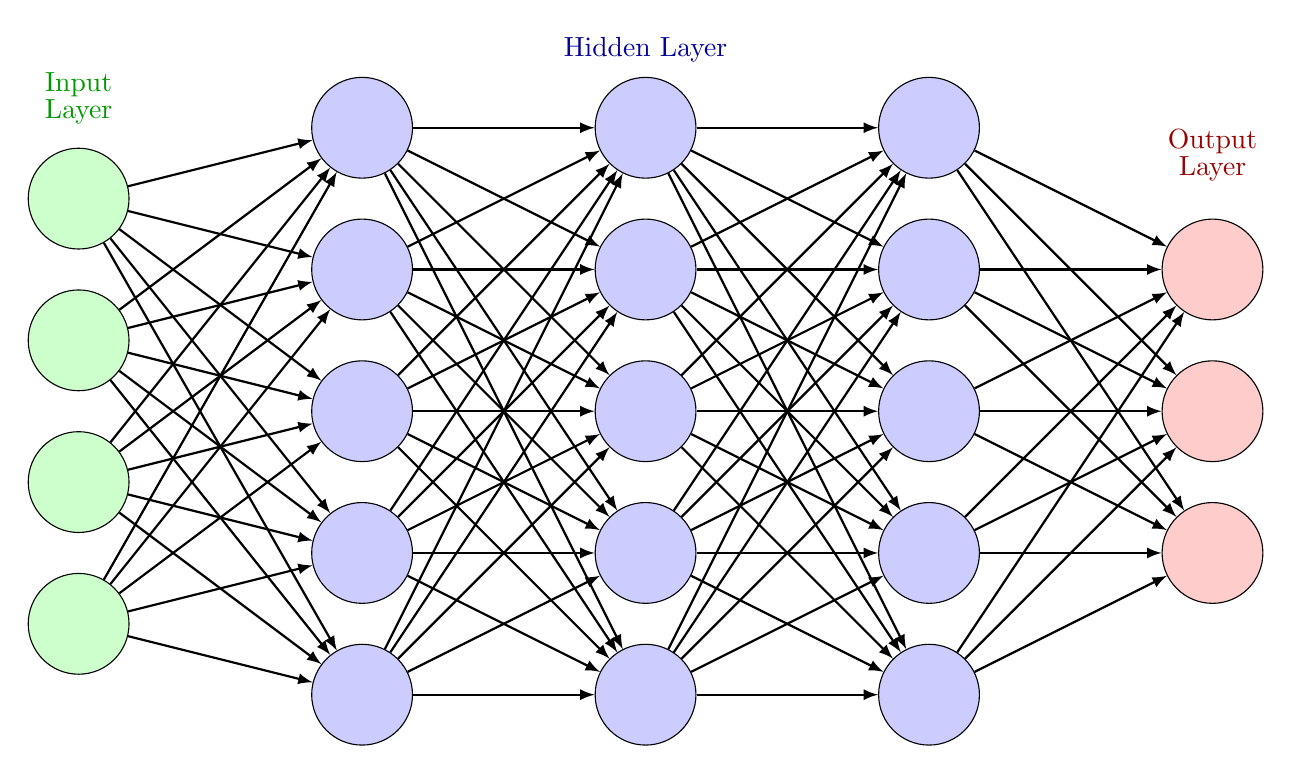
\begin{tikzpicture}[x=3.6cm,y=1.8cm]
        % Input layer (4 nodes)
        \node[node:input] (N1-1) at (1,1.5) {};
        \node[node:input] (N1-2) at (1,0.5) {};
        \node[node:input] (N1-3) at (1,-0.5) {};
        \node[node:input] (N1-4) at (1,-1.5) {};

        % First hidden layer (5 nodes)
        \node[node:hidden] (N2-1) at (2,2) {};
        \node[node:hidden] (N2-2) at (2,1) {};
        \node[node:hidden] (N2-3) at (2,0) {};
        \node[node:hidden] (N2-4) at (2,-1) {};
        \node[node:hidden] (N2-5) at (2,-2) {};

        % Second hidden layer (5 nodes)
        \node[node:hidden] (N3-1) at (3,2) {};
        \node[node:hidden] (N3-2) at (3,1) {};
        \node[node:hidden] (N3-3) at (3,0) {};
        \node[node:hidden] (N3-4) at (3,-1) {};
        \node[node:hidden] (N3-5) at (3,-2) {};

        % Third hidden layer (5 nodes)
        \node[node:hidden] (N4-1) at (4,2) {};
        \node[node:hidden] (N4-2) at (4,1) {};
        \node[node:hidden] (N4-3) at (4,0) {};
        \node[node:hidden] (N4-4) at (4,-1) {};
        \node[node:hidden] (N4-5) at (4,-2) {};

        % Output layer (3 nodes)
        \node[node:output] (N5-1) at (5,1) {};
        \node[node:output] (N5-2) at (5,0) {};
        \node[node:output] (N5-3) at (5,-1) {};

        % draw:connections from input to first hidden layer
        \foreach \i in {1,2,3,4}
        \foreach \j in {1,2,3,4,5} {
                \draw[draw:connection] (N1-\i) -- (N2-\j);
            }

        % draw:connections from first to second hidden layer
        \foreach \i in {1,2,3,4,5}
        \foreach \j in {1,2,3,4,5} {
                \draw[draw:connection] (N2-\i) -- (N3-\j);
            }

        % draw:connections from second to third hidden layer
        \foreach \i in {1,2,3,4,5}
        \foreach \j in {1,2,3,4,5} {
                \draw[draw:connection] (N3-\i) -- (N4-\j);
            }

        % draw:connections from third hidden layer to output
        \foreach \i in {1,2,3,4,5}
        \foreach \j in {1,2,3} {
                \draw[draw:connection] (N4-\i) -- (N5-\j);
            }

        % Labels
        \node[above=5,align=center,node:inputlabelcolor] at (N1-1.90) {Input\\[-0.2em]Layer};
        \node[above=2,align=center,node:hiddenlabelcolor] at (N3-1.90) {Hidden Layer};
        \node[above=10,align=center,node:outputlabelcolor] at (N5-1.90) {Output\\[-0.2em]Layer};

    \end{tikzpicture}
    \caption{Simple Neural Network}
    \label{fig:simple-neural-net}
\end{figure}

\autoref{fig:simple-neural-net} provides a simplified illustration of a simple feed-forward neural network. The network comprises four nodes in the input layer, five nodes in each of the three hidden layers, and three nodes in the output layer. Data propagate from the input layer through the network to the output layer, i.e., from left to right. The input layer contains as many nodes as the length of the input vector, whereas the output layer contains one node per quantity that the network is expected to predict. For example, if the task is to forecast a single scalar, such as carbon emissions for the next hour, a single output node suffices. Conversely, if separate forecasts are required for three successive hours, three output nodes can be retained, as illustrated in the figure. Each blue line in the diagram represents a learnable weight. When the raw feature vector is presented at the input layer, its values are multiplied by the weights of the first set of edges, summed within each hidden-layer node, shifted by a bias, and passed through a nonlinear activation function. The resulting activations are treated as a new ``feature vector'' and fed into the subsequent layer, and the process continues. Because every node in one layer is connected to every node in the next layer (i.e., the network is fully connected), it can discover interactions among any combination of input features. Intuitively, the first hidden layer detects simple patterns, while the second and third hidden layers recombine these detectors into increasingly abstract representations aligned with the final task. During training, backpropagation adjusts all weights and biases so that the outputs of the rightmost layer approximate the target values as closely as possible. At convergence, the left-to-right flow transforms the raw feature vector into a compact internal representation that is maximally informative for prediction.

In the context of neural networks, the term \emph{architecture} refers to a structural design and organization of a model. It specifies the number and types of layers, the arrangement of neurons within each layer, and the connectivity patterns among neurons. Together, these elements determine how data flow through the network and how computations are performed. This thesis focuses on the LSTM architecture. Before examining LSTMs in depth, the following sections present fundamental concepts that provide the mathematical groundwork necessary for understanding neural networks in general and the LSTM architecture in particular.

To present neural networks precisely, this thesis adopts the mathematical notation from \citetitle{goodfellow2016} by \textcite{goodfellow2016}. This thesis adopts the standard conventions: scalars (italic lowercase, e.g., \(a\), \(s\)), vectors (bold lowercase, e.g., \(\mathbf{x}\), \(\mathbf{y}\)), and matrices (bold uppercase, e.g., \(\mathbf{A}\), \(\mathbf{B}\)). Individual vector elements are accessed with subscripts (\(x_i\)), and matrix elements with row-column indices (\(A_{i,j}\)).

Having established the fundamental mathematical concepts, this thesis can now develop a precise mathematical formulation of feed-forward neural networks. This formulation will provide the necessary foundation for understanding both the forward propagation of data through the network and the subsequent backpropagation of gradients during training.

First and foremost, it is essential to understand the concept of "activation" in neural networks. Inspired by biological neurons that fire when their accumulated electrical potential exceeds a threshold, the term "activation" in artificial neural networks refers to the output value of a computational unit after processing its inputs. When a neuron produces a significant non-zero output in response to an input pattern, it is said to "activate", indicating that it has detected a feature it was trained to recognize. The mathematical function that determines this output, transforming the weighted sum of inputs into the neuron's response, is called the activation function. These functions introduce crucial nonlinearity into the network, enabling it to approximate complex relationships.

A feed-forward neural network consists of \(L\) layers, numbered from \(0\) to \(L\). Layer \(0\) is the input layer, which directly receives the feature vector representing our data point, while layer \(L\) is the output layer that produces the final prediction. The layers between, indexed as \(l \in \{1, 2, \ldots, L-1\}\), are called hidden layers because their activations are not directly observed in the input or output of the network.

Each layer \(l\) contains a certain number of units or nodes, which are denoted as \(n^{(l)}\). For example, in the context of the carbon emission forecasting task, the input layer (\(l=0\)) might have \(n^{(0)}\) of 30 nodes corresponding to different meteorological variables, energy production factors, and temporal features, while the output layer (\(l=L\)) might have \(n^{(L)}=1\) node representing the predicted carbon emissions for the next hour.

The vector of activations from layer \(l\) is denoted as \(\mathbf{h}^{(l)} \in \mathbb{R}^{n^{(l)}}\). For the input layer, these activations are simply the components of our input vector:

\[
  \mathbf{h}^{(0)} = \mathbf{x}
\]

where \(\mathbf{x} \in \mathbb{R}^{n^{(0)}}\) is the input feature vector. The vector \(\mathbf{h}^{(0)}\) passes these raw input values to the first hidden layer.

For each subsequent layer \(l \in \{1, 2, \ldots, L\}\), the computation proceeds in two steps. First, a linear transformation is calculated of the previous layer's activations, producing what is known as the pre-activation or affine transformation:

\[
  \mathbf{a}^{(l)} = \mathbf{W}^{(l)}\mathbf{h}^{(l-1)} + \mathbf{b}^{(l)}
\]

Here, \(\mathbf{W}^{(l)} \in \mathbb{R}^{n^{(l)} \times n^{(l-1)}}\) is the weight matrix for layer \(l\), and \(\mathbf{b}^{(l)} \in \mathbb{R}^{n^{(l)}}\) is the bias vector. Each element \(W^{(l)}_{i,j}\) represents the influence of the \(j\)-th unit in layer \(l-1\) on the \(i\)-th unit in layer \(l\). The bias term \(\mathbf{b}^{(l)}\) allows each unit to activate even when all inputs are zero, providing flexibility in modeling the data.

This matrix-vector multiplication computes, for each unit in layer \(l\), a weighted sum of all activations from the previous layer. Conceptually, this operation resembles a set of linear regression models, one for each unit in the current layer, with the previous layer's activations serving as predictors.

The second step in the layer-wise computation introduces nonlinearity, which is crucial for the network's ability to model complex relationships. An activation function \(g^{(l)}\) is applied element-wise to the pre-activation vector:

\[
  \mathbf{h}^{(l)} = g^{(l)}(\mathbf{a}^{(l)})
\]

The activation function \(g^{(l)}\) is typically a nonlinear function such as the sigmoid, hyperbolic tangent (tanh), or rectified linear unit (ReLU). This nonlinearity is essential because a composition of linear transformations would be a linear transformation, which would severely limit the network's expressive capacity. By introducing nonlinearities, neural networks can approximate a rich class of functions, including those with complex, non-linear relationships between inputs and outputs - precisely the type of relationships expected in carbon emission dynamics.

For the output layer \(L\), the activation function \(g^{(L)}\) is appropriate for the task at hand:

\[
  \mathbf{\hat{y}} = \mathbf{h}^{(L)} = g^{(L)}(\mathbf{a}^{(L)})
\]

where \(\mathbf{\hat{y}} \in \mathbb{R}^{n^{(L)}}\) is the network's prediction. The choice of \(g^{(L)}\) depends on the nature of the prediction task. For regression problems like forecasting carbon emissions, \(g^{(L)}\) is often the identity function, resulting in a linear output unit. For classification tasks, alternatives such as the softmax function might be more appropriate to obtain valid probability distributions over the possible classes.

The entire forward propagation process, from input to output, can be expressed as a nested function composition:

\[
  \mathbf{\hat{y}} = f(\mathbf{x}; \mathbf{\theta}) = g^{(L)}(\mathbf{W}^{(L)}g^{(L-1)}(\ldots g^{(1)}(\mathbf{W}^{(1)}\mathbf{x} + \mathbf{b}^{(1)})\ldots) + \mathbf{b}^{(L)})
\]

where \(\mathbf{\theta} = \{\mathbf{W}^{(1)}, \mathbf{b}^{(1)}, \ldots, \mathbf{W}^{(L)}, \mathbf{b}^{(L)}\}\) represents all the model parameters. This formulation highlights the sequential transformation of the input data through the network: the input vector \(\mathbf{x}\) undergoes \(L\) successive transformations, each consisting of a linear mapping followed by a nonlinear activation, eventually producing the prediction \(\mathbf{\hat{y}}\).

This mathematical expression connects directly to the earlier description of neural networks: the network ingests raw data and, layer by layer, constructs increasingly abstract representations \parencite{goodfellow2016}. The first hidden layer detects simple patterns in the input data, while subsequent hidden layers recombine these detectors into progressively more abstract representations aligned with the prediction task. At each stage, the learnable weights determine which combinations of features from the previous layer are informative for the next level of abstraction.

To understand the computation at the level of individual nodes, consider a specific unit \(i\) in layer \(l\). Its pre-activation value \(a_i^{(l)}\) is calculated as:

\[
  a_i^{(l)} = \sum_{j=1}^{n^{(l-1)}} W_{i,j}^{(l)} h_j^{(l-1)} + b_i^{(l)}
\]

This equation demonstrates how each node aggregates information from all nodes in the previous layer, weighting each input according to the learned parameters. The activation of this node is then obtained by applying the nonlinear function:

\[
  h_i^{(l)} = g^{(l)}(a_i^{(l)})
\]

This perspective aligns with the earlier description of neural networks: each node computes a weighted sum of its inputs, adds a bias term, and applies a nonlinear activation function \parencite{goodfellow2016}. The network's expressive power emerges from the collective behavior of these simple computational units arranged across multiple layers.

Given a dataset of \(m\) examples \(\{\mathbf{x}^{(1)}, \ldots, \mathbf{x}^{(m)}\}\) with corresponding targets \(\{\mathbf{y}^{(1)}, \ldots, \mathbf{y}^{(m)}\}\), the learning objective is to find the optimal parameters \(\mathbf{\theta}^*\) that minimize a loss function measuring the discrepancy between predictions and true values:

\[
  J(\mathbf{\theta}) = \frac{1}{m}\sum_{i=1}^{m}L(f(\mathbf{x}^{(i)}; \mathbf{\theta}), \mathbf{y}^{(i)})
\]

where \(J(\mathbf{\theta})\) is the overall cost function and \(L\) is the per-example loss function. For regression tasks like carbon emission forecasting, the loss function is commonly the mean squared error (MSE):

\[
  L(f(\mathbf{x}^{(i)}; \mathbf{\theta}), \mathbf{y}^{(i)}) = \|f(\mathbf{x}^{(i)}; \mathbf{\theta}) - \mathbf{y}^{(i)}\|_2^2
\]

Or more simply put:

\[
  L(\mathbf{\hat{y}}^{(i)}, \mathbf{y}^{(i)}) = \|\mathbf{\hat{y}}^{(i)} - \mathbf{y}^{(i)}\|_2^2
\]

The optimization of this objective function is typically performed using gradient-based methods, particularly the backpropagation algorithm, which efficiently computes the gradients of the cost function with respect to all parameters.

In summary, this mathematical formulation provides a precise description of how a feed-forward neural network transforms input data into predictions through a series of parameterized linear and nonlinear operations. \autoref{fig:simple-neural-net-w-notation} illustrates this process for the example architecture, where the notation shows how the input vector \(\mathbf{x}\) propagates through multiple hidden layers with associated weight matrices \(\mathbf{W}^{(l)}\) and bias vectors \(\mathbf{b}^{(l)}\) to produce the output predictions \(\mathbf{\hat{y}}\). By learning the optimal parameters that minimize the prediction error on a training dataset, the network discovers informative features and leverages them to generate accurate forecasts for complex tasks like predicting carbon emissions.

\begin{figure}[ht]
    \centering
    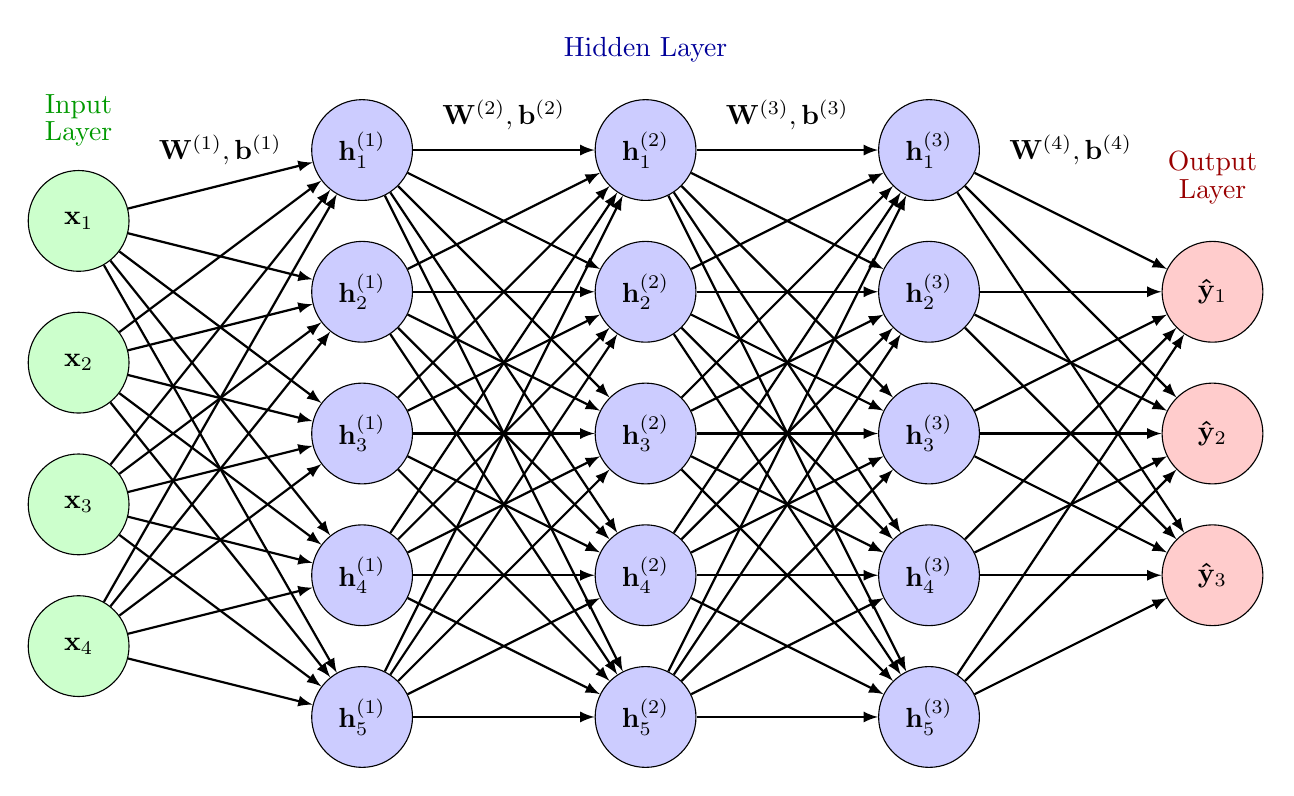
\begin{tikzpicture}[x=3.6cm,y=1.8cm]
        % Input layer (4 nodes)
        \node[node:input] (N1-1) at (1,1.5) {$\mathbf{x}_1$};
        \node[node:input] (N1-2) at (1,0.5) {$\mathbf{x}_2$};
        \node[node:input] (N1-3) at (1,-0.5) {$\mathbf{x}_3$};
        \node[node:input] (N1-4) at (1,-1.5) {$\mathbf{x}_4$};

        % First hidden layer (5 nodes)
        \node[node:hidden] (N2-1) at (2,2) {$\mathbf{h}^{(1)}_1$};
        \node[node:hidden] (N2-2) at (2,1) {$\mathbf{h}^{(1)}_2$};
        \node[node:hidden] (N2-3) at (2,0) {$\mathbf{h}^{(1)}_3$};
        \node[node:hidden] (N2-4) at (2,-1) {$\mathbf{h}^{(1)}_4$};
        \node[node:hidden] (N2-5) at (2,-2) {$\mathbf{h}^{(1)}_5$};

        % Second hidden layer (5 nodes)
        \node[node:hidden] (N3-1) at (3,2) {$\mathbf{h}^{(2)}_1$};
        \node[node:hidden] (N3-2) at (3,1) {$\mathbf{h}^{(2)}_2$};
        \node[node:hidden] (N3-3) at (3,0) {$\mathbf{h}^{(2)}_3$};
        \node[node:hidden] (N3-4) at (3,-1) {$\mathbf{h}^{(2)}_4$};
        \node[node:hidden] (N3-5) at (3,-2) {$\mathbf{h}^{(2)}_5$};

        % Third hidden layer (5 nodes)
        \node[node:hidden] (N4-1) at (4,2) {$\mathbf{h}^{(3)}_1$};
        \node[node:hidden] (N4-2) at (4,1) {$\mathbf{h}^{(3)}_2$};
        \node[node:hidden] (N4-3) at (4,0) {$\mathbf{h}^{(3)}_3$};
        \node[node:hidden] (N4-4) at (4,-1) {$\mathbf{h}^{(3)}_4$};
        \node[node:hidden] (N4-5) at (4,-2) {$\mathbf{h}^{(3)}_5$};

        % Output layer (3 nodes)
        \node[node:output] (N5-1) at (5,1) {$\mathbf{\hat{y}}_1$};
        \node[node:output] (N5-2) at (5,0) {$\mathbf{\hat{y}}_2$};
        \node[node:output] (N5-3) at (5,-1) {$\mathbf{\hat{y}}_3$};

        % draw:connections from input to first hidden layer
        \foreach \i in {1,2,3,4}
        \foreach \j in {1,2,3,4,5} {
                \draw[draw:connection] (N1-\i) -- (N2-\j);
            }

        % draw:connections from first to second hidden layer
        \foreach \i in {1,2,3,4,5}
        \foreach \j in {1,2,3,4,5} {
                \draw[draw:connection] (N2-\i) -- (N3-\j);
            }

        % draw:connections from second to third hidden layer
        \foreach \i in {1,2,3,4,5}
        \foreach \j in {1,2,3,4,5} {
                \draw[draw:connection] (N3-\i) -- (N4-\j);
            }

        % draw:connections from third hidden layer to output
        \foreach \i in {1,2,3,4,5}
        \foreach \j in {1,2,3} {
                \draw[draw:connection] (N4-\i) -- (N5-\j);
            }

        % Labels with vector notation
        \node[above=5,align=center,node:inputlabelcolor] at (N1-1.90) {Input\\[-0.2em]Layer};
        \node[above=2,align=center,node:hiddenlabelcolor] at (N3-1.90) {Hidden Layer\\[-0.2em]};
        \node[above=10,align=center,node:outputlabelcolor] at (N5-1.90) {Output\\[-0.2em]Layer};

        % Add weight matrix labels between layers
        \node[align=center] at (1.5,2) {$\mathbf{W}^{(1)}, \mathbf{b}^{(1)}$};
        \node[align=center] at (2.5,2.25) {$\mathbf{W}^{(2)}, \mathbf{b}^{(2)}$};
        \node[align=center] at (3.5,2.25) {$\mathbf{W}^{(3)}, \mathbf{b}^{(3)}$};
        \node[align=center] at (4.5,2) {$\mathbf{W}^{(4)}, \mathbf{b}^{(4)}$};
    \end{tikzpicture}
    \caption{Simple Neural Network with Notation}
    \label{fig:simple-neural-net-w-notation}
\end{figure}

As previously noted, the objective of neural network training is to minimize a loss function by systematically adjusting weights and biases to reduce prediction error. This optimization process depends on backpropagation, the central algorithm in neural network learning. By computing each parameter's contribution to the total error, backpropagation supplies precise information for updating model parameters. Forward propagation converts inputs into predictions, whereas backpropagation completes the learning loop by sending error information from the output layer back through the network, thereby directing parameter updates. Backpropagation involves a lot of math, but within the the scope of this thesis its intuition is covered instead.

At its core, backpropagation resolves the practical question of how individual weights and biases influence the overall loss. Modern networks may contain millions of parameters, making brute-force calculation infeasible. By applying the chain rule, backpropagation efficiently propagates error signals from the output layer to earlier layers, thereby obtaining partial derivatives for every parameter in a single backward pass.

The algorithm unfolds through the following steps:

\begin{enumerate}
  \item \textbf{Forward pass.} Input data traverse the network, each layer transforming the signal through its weights, biases, and activation functions. Intermediate activations are cached for later use.
  \item \textbf{Error computation.} At the output layer, the difference between the network's predictions and the target values is evaluated. For regression tasks that employ a mean squared error loss with an identity output activation, this difference is the residual between predicted and actual values.
  \item \textbf{Backward pass.} The resulting error signal propagates backward. For every layer, the algorithm assesses the contribution of each neuron to the errors in the subsequent layer. This calculation uses the transposed weight matrix, effectively reversing the direction of information flow.
  \item \textbf{Gradient calculation.} Using the propagated errors together with the stored forward activations, the algorithm computes the gradient of the loss with respect to each weight and bias. These gradients indicate the direction and magnitude of the steepest ascent of error.
  \item \textbf{Parameter update.} Finally, weights and biases are adjusted in the direction opposite to their gradients, most commonly through gradient descent or adaptive methods such as Adam or RMSprop. The learning-rate hyperparameter controls the step size of each update.
\end{enumerate}

Backpropagation is effective mainly because it is efficient \parencite{goodfellow2016}. By storing intermediate results, it computes every gradient with a cost proportional to the number of network connections. Optimization algorithms then follow these gradients, updating the weights step by step until the loss on a validation set stops improving, a signal that further training would likely lead to overfitting.

\subsection{Recurrent Neural Networks}

While feed-forward neural networks excel at learning patterns from fixed-size inputs, they cannot naturally handle sequential data where the order of observations matters. Recurrent Neural Networks (RNNs) address this limitation by introducing recurrent connections that allow information to persist across time steps. This architectural innovation makes RNNs particularly well-suited for time series forecasting applications, such as predicting carbon emissions based on historical patterns of energy generation, consumption, and meteorological conditions.

In many practical applications, including carbon emission forecasting, data arrive as sequences with temporal dependencies. For instance, the carbon emissions in DK1 at a given hour depends not only on current conditions but also on the recent history of renewable generation, demand patterns, and grid dynamics. Feed-forward networks cannot capture these temporal relationships because they process each input independently, without memory of previous inputs. RNNs overcome this limitation by maintaining an internal state that acts as a "memory" of previously processed information.

A RNN processes sequential data by iterating through the sequence elements and maintaining a state vector that is updated at each time step. Unlike feed-forward networks, which map inputs to outputs directly, RNNs share parameters across different time steps of the sequence. This parameter sharing reflects the intuition that the same rules should apply when processing each element in a sequence, regardless of its position.

While feed-forward neural networks used the superscript \((l)\) to denote different layers, RNNs use the superscript \((t)\) to denote different time steps. This change reflects the fundamental difference between these architectures: feed-forward networks process data through a spatial hierarchy of layers, while RNNs process data through a temporal sequence of steps.

\autoref{fig:rnn-unfolded} illustrates a simple RNN unfolded through time. The network processes an input sequence \(\{\mathbf{x}^{(1)},\allowbreak \mathbf{x}^{(2)},\allowbreak \mathbf{x}^{(3)}\}\) and produces a corresponding output sequence \(\{\mathbf{\hat{y}}^{(1)}, \mathbf{\hat{y}}^{(2)}, \mathbf{\hat{y}}^{(3)}\}\). At each time step \(t\), the network updates its hidden state \(\mathbf{h}^{(t)}\) based on the current input \(\mathbf{x}^{(t)}\) and the previous hidden state \(\mathbf{h}^{(t-1)}\). This recurrent connection (depicted by the horizontal arrows) enables the network to maintain information across time steps. Crucially, the same weight matrices \(\mathbf{W}_x\), \(\mathbf{W}_h\), and \(\mathbf{W}_y\) are reused at each time step, significantly reducing the number of parameters compared to a fully unfolded network with separate weights for each time step.

\begin{figure}[ht]
    \centering
    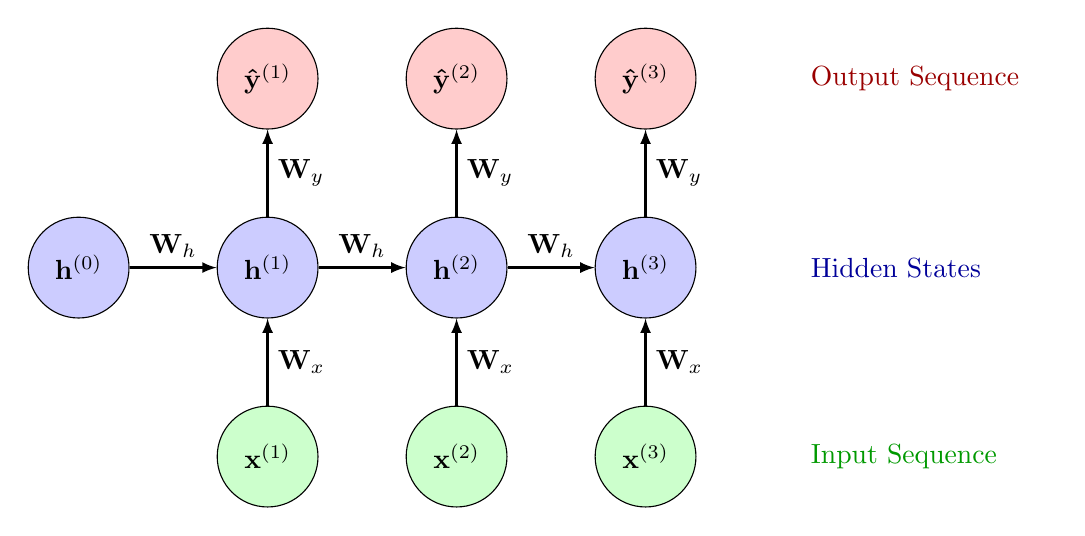
\begin{tikzpicture}[x=2.4cm,y=1.6cm]
        % Hidden states
        \node[node:hidden] (h0) at (0,0) {$\mathbf{h}^{(0)}$};
        \node[node:hidden] (h1) at (1,0) {$\mathbf{h}^{(1)}$};
        \node[node:hidden] (h2) at (2,0) {$\mathbf{h}^{(2)}$};
        \node[node:hidden] (h3) at (3,0) {$\mathbf{h}^{(3)}$};

        % Inputs
        \node[node:input] (x1) at (1,-1.5) {$\mathbf{x}^{(1)}$};
        \node[node:input] (x2) at (2,-1.5) {$\mathbf{x}^{(2)}$};
        \node[node:input] (x3) at (3,-1.5) {$\mathbf{x}^{(3)}$};

        % Outputs
        \node[node:output] (y1) at (1,1.5) {$\mathbf{\hat{y}}^{(1)}$};
        \node[node:output] (y2) at (2,1.5) {$\mathbf{\hat{y}}^{(2)}$};
        \node[node:output] (y3) at (3,1.5) {$\mathbf{\hat{y}}^{(3)}$};

        % draw:connections between hidden states
        \draw[draw:connection] (h0) -- (h1) node[midway,above] {$\mathbf{W}_{h}$};
        \draw[draw:connection] (h1) -- (h2) node[midway,above] {$\mathbf{W}_{h}$};
        \draw[draw:connection] (h2) -- (h3) node[midway,above] {$\mathbf{W}_{h}$};

        % draw:connections from inputs to hidden states
        \draw[draw:connection] (x1) -- (h1) node[midway,right] {$\mathbf{W}_{x}$};
        \draw[draw:connection] (x2) -- (h2) node[midway,right] {$\mathbf{W}_{x}$};
        \draw[draw:connection] (x3) -- (h3) node[midway,right] {$\mathbf{W}_{x}$};

        % draw:connections from hidden states to outputs
        \draw[draw:connection] (h1) -- (y1) node[midway,right] {$\mathbf{W}_{y}$};
        \draw[draw:connection] (h2) -- (y2) node[midway,right] {$\mathbf{W}_{y}$};
        \draw[draw:connection] (h3) -- (y3) node[midway,right] {$\mathbf{W}_{y}$};

        % Labels
        \node[text width=3cm,node:hiddenlabelcolor] at (4.5,0) {Hidden States};
        \node[text width=3cm,node:inputlabelcolor] at (4.5,-1.5) {Input Sequence};
        \node[text width=3cm,node:outputlabelcolor] at (4.5,1.5) {Output Sequence};

    \end{tikzpicture}
    \caption{Recurrent Neural Network Unfolded Through Time}
    \label{fig:rnn-unfolded}
\end{figure}

Consider a RNN processing a sequence of length \(T\). At each time step \(t \in \{1, 2, \ldots, T\}\), the network receives an input vector \(\mathbf{x}^{(t)} \in \mathbb{R}^{n_x}\), maintains a hidden state \(\mathbf{h}^{(t)} \in \mathbb{R}^{n_h}\), and produces an output \(\mathbf{\hat{y}}^{(t)} \in \mathbb{R}^{n_y}\).
The update equations for a basic RNN are as follows:

\[
  \mathbf{h}^{(t)} = g_h(\mathbf{W}_x\mathbf{x}^{(t)} + \mathbf{W}_h\mathbf{h}^{(t-1)} + \mathbf{b}_h)
\]
\[
  \mathbf{\hat{y}}^{(t)} = g_y(\mathbf{W}_y\mathbf{h}^{(t)} + \mathbf{b}_y)
\]

Here, \(\mathbf{W}_x \in \mathbb{R}^{n_h \times n_x}\) is the input-to-hidden weight matrix, \(\mathbf{W}_h \in \mathbb{R}^{n_h \times n_h}\) is the hidden-to-hidden weight matrix, \(\mathbf{W}_y \in \mathbb{R}^{n_y \times n_h}\) is the hidden-to-output weight matrix, and \(\mathbf{b}_h \in \mathbb{R}^{n_h}\) and \(\mathbf{b}_y \in \mathbb{R}^{n_y}\) are bias vectors \parencite{goodfellow2016}. The functions \(g_h\) and \(g_y\) are the nonlinear activation functions, which are typically hyperbolic tangent (\(\tanh\)) for the hidden state and an appropriate function for the output (identity for regression or softmax for classification).

The initial hidden state \(\mathbf{h}^{(0)}\) is typically initialized to zero or learned during training. Through recurrence relations, each hidden state \(\mathbf{h}^{(t)}\) captures information not only from the current input \(\mathbf{x}^{(t)}\) but also from all previous inputs \(\mathbf{x}^{(1)}, \mathbf{x}^{(2)}, \ldots, \mathbf{x}^{(t-1)}\). This enables the network to model temporal dependencies and patterns in sequential data.

A target variable with temporal dependencies suggest that models capable of processing sequential data would theoretically be advantageous over standard feed-forward networks, which treat each time point independently. In principle, a recurrent architecture could capture how sudden drops in wind generation lead to increased carbon emissions as fossil fuel plants compensate for the shortfall. The sequential modeling capability of RNNs appears to align well with the time series nature of carbon emission forecasting. However, electrical grid emissions are influenced by factors operating across multiple timescales, from immediate responses to renewable generation changes to longer-term effects of weather patterns and plant maintenance schedules spanning many hours or days. This multi-scale temporal dependency presents significant challenges for basic RNN architectures.

Despite their theoretical capacity to model sequential data, basic RNNs encounter fundamental limitations when applied to real-world forecasting tasks like carbon emission prediction. The key challenge emerges during training, which requires an extension of the standard backpropagation algorithm called Backpropagation Through Time (BPTT). This approach conceptually unfolds the RNN into a deep feed-forward network (as shown in \autoref{fig:rnn-unfolded}) and accumulates gradients across time steps. When learning from extended sequences, the network must propagate error signals backward through many time steps, during which gradients can either vanish (becoming too small to drive meaningful updates) or explode (growing uncontrollably and destabilizing training). This problem is particularly pronounced in RNNs because the same recurrent weights are used repeatedly during backpropagation, causing error signals to be multiplied by the same factors many times. Consequently, basic RNNs typically fail to capture long-term dependencies, precisely the type of relationships needed for accurate carbon emission forecasting, where influences may span hours or days. For instance, a morning increase in forecasted wind production might affect generation planning and carbon emissions throughout the entire day, but a standard RNN would struggle to maintain this information for sufficient time steps. These limitations motivate the development of more sophisticated RNN architectures, particularly the LSTMs introduced in the next section, which were specifically designed to overcome the vanishing gradient problem through mechanisms that help maintain and control information flow across extended time horizons.

\subsection{Long Short-Term Memory Neural Networks}

Introduced by \textcite{hochreiter1997} long short-term memory neural networks (LSTMs), represent a specialized RNN architecture designed to overcome the limitations of standard RNNs, particularly the vanishing gradient problem. While basic RNNs theoretically can learn arbitrary temporal dependencies, their practical effectiveness diminishes significantly when dealing with long-range dependencies due to the multiplicative behavior of gradients during backpropagation. LSTM networks address this fundamental limitation through a carefully engineered architecture that enables selective memory retention across extended time horizons, making them particularly suitable for tasks like carbon emission forecasting where influential factors may span hours or days.

The key innovation in LSTM networks is the introduction of a dual memory system that maintains information over arbitrary time intervals, protected and controlled by specialized gating mechanisms. Unlike standard RNN units, which overwrite their entire state at each time step, LSTM units implement two distinct types of memory that work in concert to selectively remember or forget information.

\autoref{fig:long-short-term-memory-architecture} illustrates the architecture of an LSTM unit. At the core of this architecture are two complementary memory components:

\begin{itemize}
  \item \textbf{Cell state} \(\mathbf{c}^{(t)}\): The long-term memory that acts as an information highway flowing across time steps. This component is designed to preserve important information for extended periods, potentially hundreds or thousands of time steps, with minimal degradation.
  \item \textbf{Hidden state} \(\mathbf{h}^{(t)}\): The short-term or working memory that represents what the network outputs at each time step. This component is more dynamic and reflects the network's current "focus" based on both the long-term memory and immediate inputs.
\end{itemize}

The cell state is updated through a carefully orchestrated process involving three specialized gates and a candidate value generator \parencite{hochreiter1997}:

\begin{enumerate}
  \item \textbf{Forget gate} \(\mathbf{f}^{(t)}\): Determines what information from the previous cell state should be discarded.
  \item \textbf{Candidate values} \(\mathbf{\tilde{c}}^{(t)}\): Generate new candidate information that could potentially be stored in the cell state, based on the current input and previous hidden state.
  \item \textbf{Input gate} \(\mathbf{i}^{(t)}\): Controls what portion of the candidate values will actually be stored in the cell state.
  \item \textbf{Output gate} \(\mathbf{o}^{(t)}\): Regulates what information from the updated cell state contributes to the hidden state (and thus the network's output).
\end{enumerate}

\begin{figure}[ht]
    \centering
    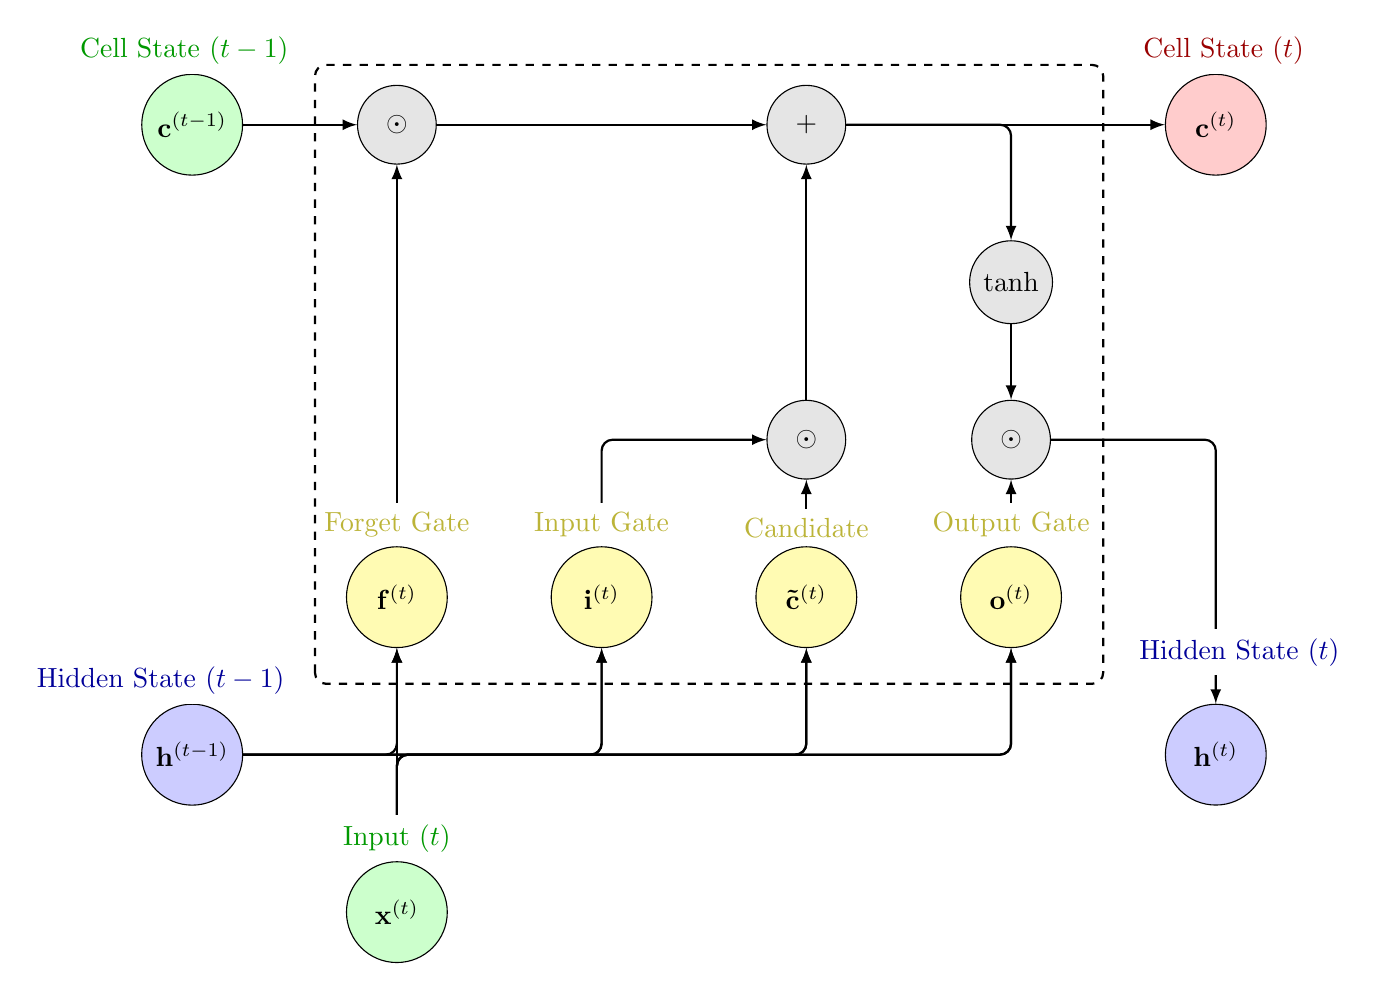
\begin{tikzpicture}[x=2.6cm, y=2cm]
        % Cell states
        \node[node:input] (c_prev) at (0,5) {$\mathbf{c}^{(t-1)}$};
        \node[node:output] (c_curr) at (5,5) {$\mathbf{c}^{(t)}$};

        % Hidden states
        \node[node:hidden] (h_prev) at (0,1) {$\mathbf{h}^{(t-1)}$};
        \node[node:hidden] (h_curr) at (5,1) {$\mathbf{h}^{(t)}$};

        % Input
        \node[node:input] (x_t) at (1,0) {$\mathbf{x}^{(t)}$};

        % Gates
        \node[node:gate] (forget) at (1,2) {$\mathbf{f}^{(t)}$};
        \node[node:gate] (input) at (2,2) {$\mathbf{i}^{(t)}$};
        \node[node:gate] (candidate) at (3,2) {$\mathbf{\tilde{c}}^{(t)}$};
        \node[node:gate] (output) at (4,2) {$\mathbf{o}^{(t)}$};

        % Operations
        \node[node:operation] (mult1) at (1,5) {$\odot$};
        \node[node:operation] (mult2) at (3,3) {$\odot$};
        \node[node:operation] (add) at (3,5) {$+$};
        \node[node:operation] (tanh) at (4,4) {$\tanh$};
        \node[node:operation] (mult3) at (4,3) {$\odot$};

        % Connections for cell state path
        \draw[draw:connection] (c_prev) -- (mult1);
        \draw[draw:connection] (mult1) -- (add);
        \draw[draw:connection] (mult2) -- (add);
        \draw[draw:connection] (add) -- (c_curr);
        \draw[draw:connection] (add) -| (tanh);

        % Connections for gates
        \draw[draw:connection] (forget) -- (mult1);
        \draw[draw:connection] (input) |- (mult2);
        \draw[draw:connection] (candidate) -- (mult2);
        \draw[draw:connection] (tanh) -- (mult3);
        \draw[draw:connection] (output) -- (mult3);
        \draw[draw:connection] (mult3) -| (h_curr);

        % Input and previous hidden state connections
        \draw[draw:connection] (h_prev) -| (forget);
        \draw[draw:connection] (h_prev) -| (input);
        \draw[draw:connection] (h_prev) -| (candidate);
        \draw[draw:connection] (h_prev) -| (output);

        \draw[draw:connection] (x_t) -- (forget);
        \draw[draw:connection] (x_t) -- ++(0,1) -- ++(1,0) -- (input);
        \draw[draw:connection] (x_t) -- ++(0,1) -- ++(2,0) -- (candidate);
        \draw[draw:connection] (x_t) -- ++(0,1) -- ++(3,0) -- (output);

        % Labels
        \node[above=0.64cm, align=center, node:inputlabelcolor, fill=white, xshift=-0.1cm] at (c_prev) {Cell State $(t-1)$};
        \node[above=0.64cm, align=center, node:outputlabelcolor, fill=white, xshift=0.1cm] at (c_curr) {Cell State $(t)$};
        \node[above=0.64cm, align=center, node:hiddenlabelcolor, fill=white, xshift=-0.4cm] at (h_prev) {Hidden State $(t-1)$};
        \node[above=1cm, align=center, node:hiddenlabelcolor, fill=white, xshift=0.3cm] at (h_curr) {Hidden State $(t)$};
        \node[above=0.64cm, align=center, node:inputlabelcolor, fill=white] at (x_t) {Input $(t)$};

        \node[above=0.64cm, align=center, node:gatelabelcolor, fill=white] at (forget) {Forget Gate};
        \node[above=0.64cm, align=center, node:gatelabelcolor, fill=white] at (input) {Input Gate};
        \node[above=0.64cm, align=center, node:gatelabelcolor, fill=white] at (candidate) {Candidate};
        \node[above=0.64cm, align=center, node:gatelabelcolor, fill=white] at (output) {Output Gate};

        % LSTM cell boundary
        \draw[dashed, rounded corners, thick] (0.60,1.45) rectangle (4.45,5.38);

    \end{tikzpicture}
    \caption{Long Short-Term Memory Neural Network Architecture}
    \label{fig:long-short-term-memory-architecture}
\end{figure}

This dual memory architecture allows the LSTM to keep important information stored for long periods in the cell state, while the hidden state can quickly adapt to new inputs. This solves the vanishing gradient problem because the cell state provides a more direct pathway for gradients to flow backward through time during training.

To describe the LSTM mathematically and better understand \autoref{fig:long-short-term-memory-architecture}, additional notation must be introduced for the gates and states involved in the computation. At each time step (t), an LSTM unit maintains two types of states: the cell state \(\mathbf{c}^{(t)} \in \mathbb{R}^{n_h}\) and the hidden state \(\mathbf{h}^{(t)} \in \mathbb{R}^{n_h}\), where \(n_h\) is the dimensionality of the hidden state.

The LSTM computation proceeds as follows:

\textbf{1. Forget gate:} The forget gate \(\mathbf{f}^{(t)}\) determines which elements of the cell state should be retained or discarded:

\[
  \mathbf{f}^{(t)} = \sigma(\mathbf{W}_f\mathbf{x}^{(t)} + \mathbf{U}_f\mathbf{h}^{(t-1)} + \mathbf{b}_f)
\]

Here, \(\mathbf{W}_f \in \mathbb{R}^{n_h \times n_x}\) and \(\mathbf{U}_f \in \mathbb{R}^{n_h \times n_h}\) are weight matrices, \(\mathbf{b}_f \in \mathbb{R}^{n_h}\) is a bias vector, and \(\sigma\) is the sigmoid activation function that outputs values between 0 and 1. Values close to 0 indicate information to forget, while values close to 1 indicate information to keep.

\textbf{2. Input gate and candidate values:} The input gate \(\mathbf{i}^{(t)}\) controls which new information will be stored in the cell state, while a \(\tanh\) layer creates a vector of candidate values \(\mathbf{\tilde{c}}^{(t)}\) that could be added to the cell state:

\[
  \mathbf{i}^{(t)} = \sigma(\mathbf{W}_i\mathbf{x}^{(t)} + \mathbf{U}_i\mathbf{h}^{(t-1)} + \mathbf{b}_i)
\]
\[
  \mathbf{\tilde{c}}^{(t)} = \tanh(\mathbf{W}_c\mathbf{x}^{(t)} + \mathbf{U}_c\mathbf{h}^{(t-1)} + \mathbf{b}_c)
\]

\textbf{3. Cell state update:} The cell state is updated by forgetting information (via the forget gate) and adding new information (via the input gate and candidate values):

\[
  \mathbf{c}^{(t)} = \mathbf{f}^{(t)} \odot \mathbf{c}^{(t-1)} + \mathbf{i}^{(t)} \odot \mathbf{\tilde{c}}^{(t)}
\]

where \(\odot\) denotes the Hadamard product (element-wise multiplication). This update equation is crucial for the LSTM's ability to maintain information over long time intervals. The multiplicative forget gate allows gradients to flow through the cell state without vanishing, as information can be preserved with minimal alteration across many time steps.

\textbf{4. Output gate and hidden state:} The output gate \(\mathbf{o}^{(t)}\) determines what information from the cell state will be exposed to the next layer or time step through the hidden state:

\[
  \mathbf{o}^{(t)} = \sigma(\mathbf{W}_o\mathbf{x}^{(t)} + \mathbf{U}_o\mathbf{h}^{(t-1)} + \mathbf{b}_o)
\]
\[
  \mathbf{h}^{(t)} = \mathbf{o}^{(t)} \odot \tanh(\mathbf{c}^{(t)})
\]

The final hidden state \(\mathbf{h}^{(t)}\) serves as both the output at the current time step and an input to the next time step.

The complete set of parameters for an LSTM layer consists of the weight matrices \(\mathbf{W}_f\), \(\mathbf{W}_i\), \(\mathbf{W}_c\), \(\mathbf{W}_o\), \(\mathbf{U}_f\), \(\mathbf{U}_i\), \(\mathbf{U}_c\), \(\mathbf{U}_o\), and the bias vectors \(\mathbf{b}_f\), \(\mathbf{b}_i\), \(\mathbf{b}_c\), \(\mathbf{b}_o\). These parameters are learned during training using backpropagation through time, as with standard RNNs \parencite{goodfellow2016}.

As with the backpropagation algorithm discussed earlier, a full mathematical revision of how LSTMs overcome the vanishing gradient problem would extend beyond the scope of this thesis. A conceptual overview provides sufficient insight into this critical advantage of LSTM networks.

The LSTM architecture addresses the vanishing gradient problem through two key mechanisms. First, the cell state acts as an information highway through which data can flow across many time steps with minimal transformation. When the forget gate outputs values close to 1, both information and gradients can propagate effectively without significant attenuation. Second, the additive update structure of the cell state (as opposed to the purely multiplicative updates in standard RNNs) prevents the gradient from being repeatedly multiplied by potentially small values during backpropagation. Together, these design elements create stable paths for gradient flow, enabling LSTMs to learn dependencies across extended time horizons.


\thispagestyle{plain}
\section{Methodology}

The Danish power grid DK1 is dominated by highly volatile wind power \parencite{iea2023,wang2017}. Consequently, the forecasting task constitutes a complex time-series problem that, as documented in the literature reviewed in \autoref{sec:lit}, is characterized by pronounced nonlinearities, strong seasonality across multiple temporal scales (hourly, daily, and yearly), and exogenous drivers such as wind speed, market demand, and cross-border electricity flows \parencite{entsoe2022}, all of which interact in a non-stationary manner \parencite{hyndman2021,box2015,carlini2023}. As indicated by the same body of literature, a promising strategy is to employ a long short-term memory neural network (LSTM) architecture \parencite{leerbeck2020,bokde2021,kohut2025,ostermann2024,lowry2018}. With the theoretical foundation just presented in \autoref{sec:theory}, this section details the methodology used to address the problem statement. Recall the main research question:

\researchquestion{}

This section presents the systematic approach employed to develop and evaluate LSTMs for carbon emission forecasting in DK1. It begins by justifying the selection of LSTM architectures, followed by detailed descriptions of data collection, feature engineering, and preprocessing procedures that prepare the dataset for modeling. The section then outlines the LSTM model architectures for both 1-hour and 24-hour forecasting horizons, establishes baseline models for comparative evaluation, describes approach to feature importance analysis, and concludes with implementation details and methodological limitations.

\subsection{Justification}

The current body of literature indicate that LSTMs are a viable modeling approach for carbon emission forecasting in volatile wind power grids \parencite{leerbeck2020,bokde2021,kohut2025,ostermann2024}. This is due to several architectural advantages that align with the temporal characteristics of electrical grid dynamics:

First, carbon emissions exhibit multi-scale temporal dependencies from immediate renewable fluctuations to longer-term weather and demand patterns \parencite{bokde2021}. LSTM gating mechanisms selectively retain relevant information across these different time horizons \parencite{goodfellow2016,hochreiter1997}.

Second, wind power generation introduces significant volatility into grid operations \parencite{wang2017, iea2023}. Sudden changes in wind conditions can trigger compensatory responses from conventional generators, affecting carbon emissions with complex lag structures \parencite{carlini2023,dong2019}. The LSTM's gating mechanisms enable it to detect these wind-related events and maintain their influence in memory for an appropriate duration \parencite{goodfellow2016}. For example, if a significant drop in wind generation typically leads to increased emissions for several hours as thermal plants ramp up, the LSTM can learn to maintain this causal relationship in its cell state.

Third, carbon emissions are influenced by a combination of deterministic patterns (such as daily load cycles) and stochastic factors (such as unexpected plant outages or forecast errors in renewable generation) \parencite{leerbeck2020}. The LSTM's flexible memory management allows it to learn which patterns are predictable and which require adaptation based on recent observations. The input gate can selectively incorporate new information that deviates from expected patterns, enabling the model to adjust its predictions in response to unusual conditions \parencite{goodfellow2016}.

Finally, the forecasting task often benefits from integrating information from multiple data streams with different temporal characteristics \parencite{leerbeck2020,kohut2025}, such as scheduled generation, weather forecasts, and historical emission measurements. The LSTM's ability to maintain a rich internal representation through its cell state enables it to effectively fuse these diverse information sources and extract the most relevant signals for prediction.

\subsection{Data Collection and Sources}

The dataset used in this thesis encompasses carbon emissions and a range of explanatory variables for the DK1 grid. Observations are of hourly resolution from January 1, 2022, to January 1, 2025, resulting in approximately 26,304 (\((365+365+366)\times24\)) observations per variable. The primary source is \href{https://www.energyquantified.com/}{Energy Quantified} (EQ), a proprietary platform that offers a comprehensive suite of data on the European energy market. EQ supplies the target variable, formally labeled "DK1 Carbon Operational Emission Power Production kgCO2eq 15min Synthetic." This variable contains historical carbon emission values from electricity generation in the DK1 grid, expressed in kilograms of carbon-dioxide equivalent (kg. \cotwoe{}). The "Synthetic" designation indicates that missing observations have been imputed with EQ's proprietary models. Besides supplying the target variable, EQ also provides a set of explanatory variables as historical forecasts. Working with forecasts rather than realized values aligns the modeling exercise with the information that is available at prediction time.

First and foremost, is power consumption in the DK1 bidding zone. This variable captures the anticipated load in the grid. DK1 operates under the merit-order/economic-dispatch principle, a ruleset provided by \citeauthor{entsoe2021} (ENTSO-E) in their paper \citetitle{entsoe2021}, where electricity generation follows an economic dispatch order with lower-cost producers dispatched before higher-cost ones. Renewables with near-zero marginal costs occupy the bottom of this supply stack, while expensive thermal units are only activated as residual demand increases \parencite{roungkvist2020}. This principle directly links electricity demand, generation mix, and resulting carbon emissions across all explanatory variables.

Besides consumption are production related variables such as solar photovoltaic production, on- and offshore wind power production, and residual production day-ahead. Solar photovoltaic and wind production forecasts are particularly critical in the DK1 context, as Denmark has one of the highest wind penetration rates globally \parencite{wang2017,iea2023}. These renewable production forecasts indicate zero-marginal-cost generation availability, while residual production day-ahead represents the anticipated thermal generation gap after accounting for renewables, directly correlating with carbon emissions. Together, these production forecasts enable the LSTM models to anticipate the supply-demand balance and the resulting dispatch order, providing essential information for accurately predicting the carbon footprint of electricity generation in the DK1 grid.

Considering more market based explanatory variables are price spot day-ahead and exchange day-ahead schedule net export. The price spot day-ahead represents the forecasted electricity price in the DK1 bidding zone for the following day, determined through the market clearing process where supply and demand curves intersect. This price variable serves as a direct indicator of the marginal generation cost required to meet demand, effectively revealing which generators are expected to be dispatched under the merit-order principle. Low electricity prices typically signal that demand can be met primarily by low-cost renewable sources \parencite{sensfuss2008}, suggesting minimal carbon emissions, while high prices indicate that expensive thermal units higher up the merit-order curve must be activated, correlating with increased carbon emissions. The price thus acts as a market-derived proxy for the carbon footprint of the generation mix \parencite{wang2017}. The exchange day-ahead schedule net export captures the planned electricity flows between DK1 and neighboring regions, reflecting the interconnected nature of the European electricity market. A positive net export indicates that DK1 expects to sell electricity to adjacent areas, suggesting abundant local generation capacity, often from wind power during favorable conditions \parencite{green2012}. Conversely, negative values (net imports) signal that DK1 anticipates importing electricity to meet local demand, which can have varying carbon implications depending on the generation mix of the exporting regions. These cross-border flows are particularly relevant for carbon emission forecasting because they affect the local supply-demand balance and can either displace local thermal generation (through imports) or indicate surplus clean generation available for export. Together, these market variables provide the LSTM models with crucial information about the economic and physical constraints that drive generator dispatch decisions, enhancing the ability of the models to predict the resulting carbon emissions in the DK1 grid.

Temperature forecasts serve as weather-driven demand indicators, as heating and cooling demands directly influence electricity consumption patterns \parencite{yao2021}, particularly in Denmark's climate where heating requirements during cold periods significantly increase consumption \parencite{cassarino2018}. Lower temperatures increase demand for carbon-intensive thermal units higher in the merit-order stack \parencite{sensfuss2008}, while milder temperatures allow renewables to meet larger proportions of reduced demand \parencite{gils2014}.

The explanatory variables described above constitute the core dataset collected from external sources and serve as the foundation for the final modeling dataset. For validation purposes, the target variable was cross-checked against the public \href{https://www.energidataservice.dk/}{Energi Data Service}, maintained by the Danish transmission system operator Energinet. This cross-validation confirmed the reliability of the EQ carbon emission data. Although Energi Data Service also provides carbon emission data and some of the explanatory variables used in this thesis, the final dataset relies exclusively on EQ data to maintain consistency across all variables and avoid potential measurement discrepancies or methodological differences between data sources. Additional predictive features, particularly time-based variables that capture temporal patterns and seasonality effects, will be systematically derived from this foundational data through feature engineering techniques, as covered in the following subsection.

\subsection{Feature Engineering}

With the current set of variables, many exogenous factors are captured. However, as the literature demonstrates, fluctuations in carbon emissions can also be attributed to time-dependent features such as hour of day, weekday, month of year, and similar temporal patterns \parencite{wang2017}. Intuitively, this relationship makes sense because carbon emissions are fundamentally linked to human behavioral patterns and consumption cycles. For example, during daytime hours, factories operate at full capacity, in the evening, families engage in cooking and household activities, and during nighttime hours, most individuals do not consume energy at significant levels. These consumption patterns are further influenced by whether it is a weekday or weekend. Therefore, to capture these temporal dependencies, time-varying variables are constructed to enable the LSTMs to associate and learn from these cyclical patterns.

The temporal feature engineering approach incorporates both linear and cyclic time representations to capture the multi-scale temporal dynamics inherent in carbon emissions data \parencite{hyndman2021}. Linear time features include hours since start, days since start, and weeks since start, which represent the elapsed time since the beginning of the dataset in different units, enabling the models to capture long-term trends and drift patterns. Additionally, year and year-month variables provide yearly and monthly progression information to account for long-term trends and seasonal variations at the annual scale.

To effectively represent the inherently cyclical nature of temporal patterns, sine and cosine transformations are employed for various time periods. The hourly cycle is captured through hourly sine and cosine variables, which encode the 24-hour daily rhythm that reflects diurnal energy consumption patterns, such as peak demand during business hours and minimal usage during overnight periods. Weekly patterns are represented by daily sine and cosine variables, capturing the distinction between weekday and weekend consumption behaviors. Monthly cycles are encoded via monthly sine and cosine variables to account for seasonal variations in energy demand, such as increased heating requirements during winter months. Finally, quarterly sine and cosine variables capture quarterly business and economic cycles that may influence industrial energy consumption patterns \parencite{yasmeen2022}. This cyclic feature engineering approach ensures that temporal relationships are preserved across period boundaries, allowing the LSTMs to recognize that the end of one cycle naturally transitions to the beginning of the next.

The final dataset has been constructed incorporating both exogenous variables and time-dependent features. For a comprehensive overview of the complete dataset and the associated variable names, see \autorefapdx{apdx:final-dataset}.

\subsection{Data Preprocessing}

Prior to model training, the assembled dataset underwent several preprocessing steps to ensure data quality and compatibility with the LSTM architectures. The data provided by EQ contained no missing values, eliminating the need for imputation procedures. This data completeness is attributable to EQ's proprietary synthetic data generation methods. The target variable was converted from kilograms to tonnes of \cotwoe to enhance interpretability and enable comparison with findings reported in the existing literature.

All observations were ordered chronologically from oldest to newest to maintain the temporal sequence essential for time series modeling. The dataset was then split into training, validation, and test sets using a 70/15/15 ratio, with validation and test periods following the training period chronologically. This temporal split prevents data leakage that could occur with random sampling approaches by ensuring that models only utilize historical information available at prediction time, closely mimicking operational forecasting scenarios \parencite{cerqueira2020,tashman2000}. The test set remains strictly held out throughout the entire model development process and is used exclusively for final performance evaluation.

To address the varying scales and units across the feature set, all variables underwent min-max normalization, scaling each feature to a range between zero and one. This normalization step is particularly important for neural network training, as it ensures that variables with larger absolute values do not dominate the learning process and helps maintain stable gradient flows during backpropagation \parencite{goodfellow2016}. The scaling parameters were fitted exclusively on the training set and subsequently applied to the validation and test sets to prevent information leakage from future observations into the model training process.

Outlier detection and removal procedures were deliberately omitted to preserve the integrity of the temporal sequence and maintain realistic operating conditions within the dataset. In the context of electrical grid operations, extreme values in carbon emissions often represent legitimate operational scenarios such as unexpected plant outages, grid emergencies, or periods of low renewable generation that require rapid deployment of backup thermal capacity. Removing such observations would eliminate precisely the challenging conditions that the forecasting models must learn to handle in real-world deployment. Furthermore, the LSTM architecture's gating mechanisms provide inherent robustness to occasional extreme values while preserving the temporal continuity essential for learning sequential patterns \parencite{goodfellow2016}.

\subsection{LSTM Model Architectures}
\label{subsec:lstm-model-architecture}

This thesis focuses on short-term CO2 emission forecasting with a target horizon of 1--24 hours, a timeframe that aligns with the practical use cases outlined in the introduction \parencite{entsoe2022,futurebridge}. To systematically evaluate the effectiveness of LSTMs for carbon emission prediction, two distinct architectures are developed. The first architecture targets a simpler 1-hour ahead forecasting task (output \(\hat{y}^{(t+1)}\)), while the second addresses the primary research objective of 24-hour ahead prediction (output \(\mathbf{\hat{y}}^{(t+1:t+24)}\)). This approach allows to first gain understanding and insights with LSTM performance on this specific forecasting problem through a less complex prediction task. The learnings acquired from the first model can then inform the design decisions for the 24-hour architecture. However, each architecture will be developed independently, with hyperparameters such as LSTM units, input sequence length, learning rate, and batch size explored separately to optimize performance for their respective forecasting horizons.

Beyond hyperparameters, several fundamental architectural and training decisions must be established for the LSTM implementations. These decisions can be categorized into those that can be determined prior to model training based on theoretical considerations and problem characteristics, and those that require empirical exploration through the training process. This subsection first addresses the former category, establishing the core training configuration choices that form the foundation of the LSTM architectures, before outlining a systematic framework for exploring the empirical architectural decisions that require experimental evaluation.

Mean squared error (MSE), as presented in \autoref{sec:theory}, is employed as the loss function for this regression task, providing differentiable gradients for stable LSTM optimization \parencite{goodfellow2016}. The Adam optimizer is employed for backpropagation due to its demonstrated effectiveness with time series data \parencite{makinde2024}, adaptive learning rates for each parameter, and robust convergence properties suitable for complex temporal dependencies in grid data \parencite{chang2018}.

Two callback mechanisms enhance training stability: early stopping (patience of five epochs) prevents overfitting by terminating training when validation loss stagnates, while a learning rate scheduler reduces the rate by 0.5 after three epochs without improvement (minimum 0.00001). This addresses LSTM training challenges where fixed learning rates prevent fine-tuning, allowing models to train until convergence rather than for a predetermined epoch count \parencite{goodfellow2016}.

The 1-hour and 24-hour forecasting tasks employ distinct architectural approaches tailored to their respective prediction complexities and horizons. For the 1-hour ahead forecasting task, a single-layer LSTM configuration is implemented. This design choice is justified by the relatively straightforward nature of single-step prediction, where the model outputs a scalar value (\(\hat{y}^{(t+1)}\)) representing carbon emissions one hour into the future. The single-layer architecture provides sufficient modeling capacity for this prediction horizon while minimizing computational complexity and reducing overfitting risk \parencite{greff2017}. In contrast, the 24-hour ahead forecasting task employs an encoder-decoder architecture to address the inherent complexity of multi-step sequence prediction. This design choice is motivated by several factors specific to the 24-hour forecasting challenge. First, the encoder-decoder architecture naturally accommodates the sequence-to-sequence nature of generating 24 consecutive hourly predictions (\(\mathbf{\hat{y}}^{(t+1:t+24)}\)), where the encoder processes historical time series data to create a compressed representation, and the decoder generates the multi-step forecast sequence \parencite{sutskever2014}. Second, this architecture effectively handles the integration of both historical features and future exogenous variables, such as consumption forecasts, which are available at prediction time and crucial for accurate long-term forecasting. Finally, the encoder-decoder architecture addresses the increased complexity of multi-step ahead prediction by providing dedicated components for feature extraction and sequence generation, enabling the model to capture both long-term temporal dependencies and the evolving patterns across the 24-hour prediction horizon \parencite{he2024}.

The hyperparameter optimization follows a coordinate descent approach designed to efficiently explore the hyperparameter space within computational constraints. The procedure begins by randomly selecting initial values from the predefined ranges specified in \autoref{tab:hyperparameter-ranges-lstm} to establish a starting configuration \parencite{bergstra2018}. Subsequently, each hyperparameter is optimized individually while holding others constant, following the sequence: number of LSTM units, input sequence length, learning rate, and batch size.

\begin{table}[ht]
  \centering
  \begin{tabular}{lc}
    \hline
    \textbf{Hyperparameter} & \textbf{Values}          \\ \hline
    Number of LSTM units    & 16, 32, 64, 128, 256     \\
    Input sequence length   & 24, 48, 72, 96           \\
    Learning rate           & .01, .001, .0001, .00001 \\
    Batch size              & 16, 32, 64, 128, 256     \\ \hline
  \end{tabular}
  \caption{Hyperparameter Values for LSTM Models Exploration}
  \label{tab:hyperparameter-ranges-lstm}
\end{table}

For each hyperparameter, the optimization explores adjacent values in a hill-climbing manner. Starting from the current value, the procedure evaluates neighboring options (e.g., if currently using 32 LSTM units, testing both 16 and 64 units) and selects the configuration that yields the lowest validation RMSE. If improvement is observed, the search continues in that direction until no further improvement is achieved. If no improvement is found in either direction, the current value is retained as optimal for that hyperparameter. This process ensures systematic exploration while avoiding exhaustive grid search.

Following the individual hyperparameter optimization, a final validation phase conducts random perturbations across all hyperparameters simultaneously to identify potential hyperparameter interactions that the coordinate descent approach might miss. This two-stage procedure balances computational efficiency with thorough exploration, ensuring robust hyperparameter selection for both the 1-hour and 24-hour forecasting architectures.

The combination of theoretically justified design choices and systematic manual hyperparameter tuning provides a robust foundation for developing optimal LSTM architectures tailored to the specific characteristics of carbon emission forecasting in the DK1 grid.

\subsection{Detailed Encoder-Decoder Architecture}

The encoder-decoder architecture for 24-hour forecasting is specifically designed to leverage both historical time series patterns and future exogenous variable forecasts available at prediction time. The encoder processes historical observations \((\mathbf{x}^{(t-L+1)}, \mathbf{x}^{(t-L+2)}, \ldots, \mathbf{x}^{(t)})\) to create compressed representations of temporal patterns, while the decoder generates the 24-hour prediction sequence \((\mathbf{\hat{y}}^{(t+1:t+24)})\) using both encoder output and future exogenous variable forecasts \(\mathbf{x}^{(t+h)}\) available at prediction time. This design directly addresses the merit-order by incorporating forecasted renewable generation, consumption, and market variables that determine the expected dispatch order and resulting carbon emissions. The decoder architecture mirrors the encoder in terms of LSTM units but includes an additional dense layer with linear activation to produce the carbon emission prediction at each time step.

This architectural choice is particularly well-suited to the DK1 forecasting task because EQ provides 24-hour ahead forecasts for all explanatory variables at prediction time, simulating the realistic operational scenario where grid operators have access to day-ahead explanatory variables when making carbon emission predictions.

\subsection{Baseline Models and Evaluation}

To assess the performance of the LSTM architectures, two baseline models are employed for comparative evaluation: a naive persistence model and an Autoregressive Integrated Moving Average (ARIMA) model. Each baseline is developed for both the 1-hour and 24-hour forecasting horizons. The naive persistence model represents the simplest forecasting approach, where future values are assumed to equal the most recent observation. For the 1-hour forecasting task, this translates to \(\hat{y}^{(t+1)} = y^{(t)}\), where the predicted carbon emissions one hour ahead equal the current observed value. For the 24-hour forecasting horizon, the naive model extends this logic across the entire prediction sequence, such that \(\hat{y}^{(t+h)} = y^{(t)}\) for \(h \in \{1, 2, \ldots, 24\}\), meaning all future hourly predictions are set equal to the current carbon emission level.

The ARIMA model serves as a traditional time series forecasting baseline that captures linear temporal dependencies through autoregressive, differencing, and moving average components. To ensure optimal ARIMA performance, a systematic grid search is conducted across all combinations of parameters: autoregressive order (\(p\)) from 0 to 5, differencing order (\(d\)) from 0 to 2, moving average order (\(q\)) from 0 to 5, and trend specifications including none, constant, and linear trends. The best-performing ARIMA configuration is selected based on out-of-sample validation RMSE. This results in six distinct models for comparison: two LSTM architectures, two naive baselines, and two optimally-configured ARIMA models, each tailored to their respective forecasting horizons.

These baseline models provide complementary benchmarks for evaluating the LSTMs. The naive models serve as a fundamental threshold that any forecasting model must surpass to demonstrate value, while the ARIMA models represent the established statistical approach capable of capturing linear temporal dependencies and trends. Together, they create a range from minimal sophistication to traditional time series modeling, enabling assessment of whether the LSTM architectures can justify their computational complexity by capturing the complex nonlinear relationships between renewable generation, grid dynamics, and carbon emissions that simpler linear approaches cannot effectively model.

The performance of all forecasting models is evaluated using Root Mean Squared Error (RMSE) as the primary evaluation metric, calculated as:

\[
  RMSE = \sqrt{\frac{1}{m}\sum_{i=1}^{m}\|\mathbf{\hat{y}}^{(i)} - \mathbf{y}^{(i)}\|_2^2}
\]

where \(m\) represents the number of test examples. RMSE serves as the primary comparison metric for determining LSTM superiority over baseline models because its quadratic penalty structure emphasizes larger prediction errors, aligning with the operational reality that substantial forecasting errors in carbon emissions carry disproportionately severe consequences for grid planning and regulatory compliance. Additionally, RMSE maintains the same units as the target variable, facilitating intuitive interpretation of forecasting accuracy.
Mean Absolute Error (MAE) provides complementary evaluation insight, defined as:

\[
  MAE = \frac{1}{m}\sum_{i=1}^{m}\|\mathbf{\hat{y}}^{(i)} - \mathbf{y}^{(i)}\|_1
\]

MAE offers equal weight to all prediction errors and reduced sensitivity to outliers, providing additional understanding of typical forecasting performance under normal operating conditions.

To ensure that RMSE improvements achieved by LSTM models represent statistically significant advances over baseline approaches rather than random variation, the Diebold-Mariano test is employed for pairwise forecast accuracy comparisons. This test is specifically designed for comparing predictive accuracy of competing forecasting models and accounts for the potential correlation in forecast errors that arises from using the same underlying dataset. The test statistic is calculated based on the RMSE loss differential series between competing models, where the null hypothesis assumes equal predictive accuracy. The test is applied to compare LSTM performance against each baseline model (naive persistence and ARIMA) for both forecasting horizons, using a two-sided test at a significance level of \(\alpha = 0.05\). Rejection of the null hypothesis indicates that the observed RMSE differences are statistically significant rather than attributable to random variation in the test set \parencite{diebold1995}.

This statistical validation is particularly important for carbon emission forecasting applications where model deployment decisions must be justified based on demonstrable performance improvements that exceed measurement uncertainty and natural variability in grid operations. The combination of RMSE-based performance comparison and Diebold-Mariano statistical testing provides robust assessment of whether the increased computational complexity of LSTM models translates into meaningful and statistically significant improvements in carbon emission prediction accuracy.

\subsection{Feature Importance Analysis}

To validate the relevance of the selected explanatory variables and feature engineering choices, permutation importance analysis is conducted on the trained 24-hour LSTM model. This analysis provides empirical insight into which features contribute most significantly to the model's predictive performance and confirms whether the theoretical justifications for variable selection align with the model's actual learning behavior \parencite{altmann2010}.

Permutation importance operates by systematically shuffling the values of each feature in the validation set while keeping all other features unchanged, then measuring the resulting degradation in model performance. The importance score for each feature is calculated as the difference between the baseline validation RMSE and the RMSE obtained after permuting that feature's values. For each feature, the permutation process is repeated 10 times with different random seeds to ensure robust importance estimates \parencite{altmann2010}. This approach is particularly suitable for LSTM architectures because it treats the model as a black box, avoiding the need to interpret complex internal states while naturally handling temporal dependencies in the input sequences.

The analysis focuses exclusively on the 24-hour LSTM model due to its primary practical relevance for the operational use cases outlined in the introduction and its more comprehensive feature set that includes both historical patterns and future exogenous variable forecasts. The analysis encompasses both the original exogenous variables collected from EQ and the engineered temporal features.

This permutation importance analysis serves three key validation purposes: confirming whether variables identified as conceptually important based on merit-order principles actually contribute to model performance, revealing the relative importance of different feature categories (supply-side versus demand-side variables), and assessing the contribution of engineered time-based patterns relative to domain-specific grid variables. These insights enhance the interpretability of the LSTM model and provide confidence in how the architecture leverages available information for carbon emission forecasting in the DK1 grid.

\subsection{Implementation Details}

The full implementation from data retrieval to modeling has been done using Python. All the source code is provided in a zip-file as additional material. For an overview of the different components see \autorefapdx{apdx:code-overview}. Most notably, data was extracted via \href{https://energyquantified-python.readthedocs.io/}{EQs Time Series API }, transformed using \href{https://pola.rs/}{Polars}, and finally modelled using \href{https://www.tensorflow.org/}{TensorFlow} - one of the most popular libraries for working with neural networks.

\subsection{Limitations}

While this methodology provides a focused approach to carbon emission forecasting in DK1, several design choices impose boundaries on the scope and generalizability of findings.

The exclusive focus on LSTM networks excludes evaluation of other promising sequential architectures identified in the literature. Alternatives such as gated recurrent units (GRUs), temporal convolutional networks (TCNs), and Transformer-based encoders offer different approaches to modeling temporal dependencies. This architectural limitation prevents direct comparison of LSTM performance against these potentially suitable alternatives for carbon emission forecasting.

Despite substantial literature evidence that hybrid statistical-machine learning approaches consistently outperform standalone models, this thesis focuses exclusively on pure LSTM architectures compared to traditional baselines. The literature reviewed in \autoref{sec:lit} demonstrates that ARIMA-LSTM combinations frequently achieve superior accuracy to either method individually, yet this methodology deliberately excludes such hybrid approaches to maintain focus on evaluating standalone LSTM capabilities. Similarly, the comparative evaluation is limited to naive persistence and ARIMA models, excluding other machine learning baselines such as random forests, gradient boosting, or support vector regression that the literature suggests can be competitive for energy forecasting tasks.

The DK1-focused dataset, while addressing an identified research gap, may limit generalizability to other renewable-dominated grids with different operational characteristics, market structures, or renewable penetration levels. The unique wind-heavy profile of DK1 may not represent patterns applicable to other regional contexts. Additionally, the reliance on EQ's proprietary gap-filling methods introduces potential unknown biases into the dataset. While this ensures completeness, the synthetic data generation process may alter natural patterns in ways that could influence model learning and evaluation.

The 70/15/15 temporal split allocates the majority of historical observations to training, with validation and test sets representing the most recent periods of the dataset. While this split maintains chronological ordering essential for time series evaluation, the test period's position at the end of the dataset means that final performance evaluation reflects the model's ability to predict carbon emissions during the most recent operational period. This recent period may exhibit different patterns from earlier historical periods due to evolving grid infrastructure, policy changes, or market dynamics, potentially limiting the representation of seasonal variations across the full dataset timeframe. This temporal limitation is inherent to time series forecasting evaluation but should be considered when interpreting the generalizability of performance results to future operational periods that may extend beyond the characteristics captured in the training data.


\thispagestyle{plain}
\section{Results}
\label{sec:results}

This section presents the empirical findings from the carbon emission forecasting models developed according to the methodology outlined in the previous section. The analysis unfolds systematically to evaluate both forecasting performance and findings across the prediction horizons.

Baseline model results establish the performance thresholds that the long short-term memory neural network (LSTM) architectures must exceed to demonstrate value. The investigation then advances through the LSTM implementations, examining hyperparameter optimization and training dynamics for both 1-hour and 24-hour forecasting tasks. Beyond predictive accuracy, the analysis dives deeper into the 24-hour LSTM through feature importance analysis, revealing which variables drive forecasting performance and validating the theoretical foundations underlying variable selection. Note that all error figures, such as Root Mean Squared Error (RMSE) and Mean Absolute Error (MAE), are reported in tonnes \cotwoe{} unless otherwise stated.

\subsection{Baseline Model Performance}

Four baseline models were established to provide comparative benchmarks for evaluating LSTM performance across both forecasting horizons. The naive persistence models assume that future carbon emissions equal the most recent observed value, implemented as \(\hat{y}^{(t+1)} = y^{(t)}\) for the 1-hour horizon and \(\hat{y}^{(t+h)} = y^{(t)}\) for \(h \in \{1, 2, \ldots, 24\}\) in the 24-hour forecasting task.

For the ARIMA models, systematic grid search optimization was conducted across all parameter combinations as specified in the methodology. The optimal configuration for both forecasting horizons was identified as ARIMA(5,0,5) with no trend component, indicating that an autoregressive order of 5, no differencing, and a moving average order of 5 provided the best out-of-sample validation performance for both the 1-hour and 24-hour prediction tasks.

The final test set evaluation revealed substantial performance differences across models and forecasting horizons. For the 1-hour ahead forecasting task, the naive persistence model achieved a test RMSE of 10.54 and MAE of 6.13, while the ARIMA(5,0,5) model demonstrated improved performance with an RMSE of 9.43 and MAE of 5.99. The 24-hour forecasting horizon presented considerably greater prediction complexity, with the naive persistence model yielding a test RMSE of 29.75 and MAE of 20.33, and the ARIMA(5,0,5) model achieving an RMSE of 25.03 and MAE of 18.21.

To validate the statistical significance of these performance differences, two-sided Diebold-Mariano tests were conducted comparing ARIMA against naive persistence models for both forecasting horizons. The tests confirmed statistically significant improvements, with p-values effectively zero for both the 1-hour (DM statistic: -12.12) and 24-hour (DM statistic: -16.15) comparisons, enabling rejection of the null hypothesis of equal predictive accuracy at the \(\alpha = 0.05\) significance level.

The consistent pattern of ARIMA outperforming naive persistence across both RMSE and MAE metrics, validated through statistical testing, confirms the value of capturing linear temporal dependencies in carbon emission patterns. However, the substantial increase in error magnitudes from 1-hour to 24-hour forecasting horizons across both evaluation metrics underscores the inherent difficulty of extended prediction periods in volatile wind power grids. These baseline results establish the performance thresholds that the LSTM architectures must exceed to demonstrate meaningful forecasting improvements.

\subsection{LSTM Hyperparameter Optimization and Training Results}

Following the coordinate descent approach outlined in the methodology, systematic hyperparameter optimization was conducted for both LSTM architectures. The optimization procedure explored the hyperparameter space defined in the methodology across number of LSTM units, input sequence length, learning rate, and batch size, with each parameter optimized individually while holding others constant to identify optimal configurations for both forecasting horizons.

For the 1-hour ahead forecasting task, the single-layer LSTM architecture achieved optimal performance with 32 LSTM units processing an input sequence length of 48 hours. The model training employed a learning rate of 0.0001 with a batch size of 16, converging after 25 epochs through the early stopping mechanism. This configuration yielded a final test performance of 9.01 RMSE and 6.28 MAE, demonstrating the model's ability to capture short-term temporal dependencies in carbon emission patterns.

The 24-hour ahead forecasting task utilizing the encoder-decoder architecture identified an optimal configuration with 32 LSTM units in both encoder and decoder components, maintaining the same 48-hour input sequence length as the 1-hour model. The training process employed an identical learning rate of 0.0001, though with an increased batch size of 64 to accommodate the more complex sequence-to-sequence learning task. Training convergence occurred after 25 epochs, resulting in test performance of 22.20 RMSE and 16.32 MAE across the 24-hour prediction horizon.

The architectural differences between the two models reflect their distinct prediction requirements. The 1-hour model's single-layer LSTM configuration proved sufficient for the scalar output prediction task, while the 24-hour model's encoder-decoder architecture enabled effective processing of both historical temporal patterns and future exogenous variable forecasts. Notably, both models converged to similar hyperparameter values for LSTM units, input sequence length, and learning rate, suggesting consistent optimal learning characteristics across the different architectural approaches. The primary distinction emerged in batch size requirements, where the encoder-decoder model benefited from larger batch sizes to stabilize the more complex gradient computations inherent in sequence-to-sequence learning.

Training stability was achieved for both architectures through the implemented callback mechanisms. The early stopping criterion prevented overfitting by monitoring validation loss with a patience of five epochs, while the learning rate scheduler enabled fine-tuning through plateau-based reductions. Both models demonstrated smooth convergence behavior without oscillations or instability, indicating that the selected hyperparameter configurations and training procedures were well-suited to the carbon emission forecasting task in the DK1 grid context.

\begin{figure}[ht]
  \centering
  \includegraphics[width=10cm]{sections/figures/lstm_point_model_loss_during_training.png}
  \caption{LSTM 1-hour Model Loss During Training}
  \label{fig:lstm-point-model-loss-during-training}
\end{figure}

\begin{figure}[ht]
  \centering
  \includegraphics[width=10cm]{sections/figures/lstm_seq_model_loss_during_training.png}
  \caption{LSTM 24-hour Model Loss During Training}
  \label{fig:lstm-seq-model-loss-during-training}
\end{figure}

The training dynamics are illustrated in the loss curves for both architectures (\autoref{fig:lstm-point-model-loss-during-training} and \autoref{fig:lstm-seq-model-loss-during-training}), which exhibit the expected convergence patterns for well-configured LSTM models. Both the 1-hour and 24-hour models show rapid initial loss reduction during the first few epochs, followed by gradual convergence toward optimal performance levels. The training and validation losses track closely throughout the optimization process, with validation loss remaining slightly higher than training loss as expected, demonstrating effective generalization without significant overfitting. The absence of divergence between training and validation curves confirms that the models learned meaningful temporal patterns rather than memorizing training sequences, validating the robustness of the selected hyperparameter configurations for carbon emission forecasting in volatile wind power grids.

\subsection{LSTM Forecasting Results}

Following the hyperparameter optimization and training procedures outlined in the previous subsection, this section presents a comprehensive evaluation of LSTM forecasting performance across both prediction horizons. The analysis proceeds through residual diagnostics to assess model behavior and prediction quality, followed by performance comparisons against the established baseline models and statistical significance testing to validate the empirical improvements achieved by the LSTM architectures.

The residual analysis provides essential insights into model performance characteristics and potential systematic biases. For the 1-hour LSTM model, the residual distribution (\autoref{fig:lstm-point-test-residuals-frequency}) exhibits a approximately normal distribution centered near zero, indicating unbiased predictions with no systematic over- or under-prediction tendencies. The residual spread ranges primarily between -40 and +40 tonnes \cotwoe{}, with the majority of prediction errors concentrated within ±20 tonnes, demonstrating reasonable prediction accuracy for short-term forecasting applications. The temporal pattern of residuals (\autoref{fig:lstm-point-test-residuals-over-time}) reveals no obvious systematic trends or seasonal patterns in the errors, confirming that the model effectively captures the underlying temporal dependencies in carbon emission patterns without exhibiting time-dependent bias.

\begin{figure}[ht]
  \centering
  \includegraphics[width=10cm]{sections/figures/lstm_point_test_residuals_frequency.png}
  \caption{LSTM 1-hour Model Test Residuals Frequency}
  \label{fig:lstm-point-test-residuals-frequency}
\end{figure}

\begin{figure}[ht]
  \centering
  \includegraphics[width=10cm]{sections/figures/lstm_point_test_residuals_over_time.png}
  \caption{LSTM 1-hour Model Test Residuals Over Time}
  \label{fig:lstm-point-test-residuals-over-time}
\end{figure}

The 24-hour LSTM model demonstrates similar residual characteristics, though with appropriately larger error magnitudes reflecting the increased complexity of an extended forecasting horizon. The residual distribution (\autoref{fig:lstm-seq-test-residuals-frequency}) maintains a near-normal distribution centered at zero, with residuals primarily ranging between -75 and +75 tonnes \cotwoe{}. While the error spread is approximately double that of the 1-hour model, this increase is proportionally reasonable given the substantially longer prediction horizon and the cumulative uncertainty inherent in multi-step forecasting. The temporal residual pattern (\autoref{fig:lstm-seq-test-residuals-over-time}) similarly shows no systematic temporal bias, indicating effective learning of long-term dependencies across the 24-hour prediction sequences.

\begin{figure}[ht]
  \centering
  \includegraphics[width=10cm]{sections/figures/lstm_seq_test_residuals_frequency.png}
  \caption{LSTM 24-hour Model Test Residuals Frequency}
  \label{fig:lstm-seq-test-residuals-frequency}
\end{figure}

\begin{figure}[ht]
  \centering
  \includegraphics[width=10cm]{sections/figures/lstm_seq_test_residuals_over_time.png}
  \caption{LSTM 24-hour Model Test Residuals Over Time}
  \label{fig:lstm-seq-test-residuals-over-time}
\end{figure}

Representative prediction examples (shown in \autorefapdx{apdx:lstms-predictions-vs-actuals}) illustrate the practical forecasting capabilities of both LSTM architectures. The 1-hour model predictions (\autoref{fig:lstm-point-test-pred-vs-acts}) demonstrate close tracking of actual carbon emission patterns across various operational scenarios, capturing both gradual trends and more volatile fluctuations characteristic of wind-dominated grids. The model effectively follows the directional changes in emissions while maintaining reasonable accuracy during periods of rapid variation. For the 24-hour model (\autoref{fig:lstm-seq-test-pred-vs-acts}), the sequence predictions show strong performance in capturing overall emission trends and patterns across the full prediction horizon. While some divergence between predicted and actual values becomes apparent in the later hours of certain sequences, the model generally maintains directional accuracy and captures the fundamental emission patterns driven by renewable generation variability and demand cycles.

Comparative performance evaluation reveals substantial improvements over baseline approaches across both forecasting horizons. For 1-hour-ahead prediction, the LSTM model achieved a test RMSE of 9.01 and MAE of 6.28, representing a 14.5\% decrease in RMSE compared with the naive persistence baseline (RMSE = 10.54, MAE = 6.13), albeit with a 2.4\% increase in MAE. Relative to the ARIMA model (RMSE = 9.43, MAE = 5.99), the LSTM delivered a 4.5\% decrease in RMSE while showing a 4.8\% increase in MAE. The 24-hour forecasting results are even more pronounced: the LSTM obtained an RMSE of 22.20 and MAE of 16.32, corresponding to decreases of 25.4\% in RMSE and 19.7\% in MAE over naive persistence (RMSE = 29.75, MAE = 20.33). Compared with the ARIMA benchmark (RMSE = 25.03, MAE = 18.21), the LSTM achieves decreases of 11.3\% in RMSE and 10.4\% in MAE. For a comprehensive overview of all model error metrics across train, test, and validation splits see \autoref{tab:overview-maes-across-models} and \autoref{tab:overview-rmse-across-models} in \autorefapdx{apdx:comprehensive-model-error-metrics}.

Statistical significance testing through two-sided Diebold-Mariano tests confirms that these performance improvements represent meaningful advances rather than random variation. For the 1-hour forecasting task, the LSTM significantly outperformed both the naive baseline (DM statistic = -10.05, \(p < 0.0001\)) and the ARIMA model (DM statistic = -3.67, \(p = 0.0002\)), enabling rejection of the null hypothesis of equal predictive accuracy. The 24-hour results show even stronger statistical evidence, with the LSTM demonstrating highly significant improvements over naive persistence (DM statistic = -19.12, \(p < 0.0001\)) and ARIMA (DM statistic = -9.65, \(p < 0.0001\)). These results provide robust statistical validation that the LSTM architectures deliver substantially improved carbon emission forecasting accuracy for volatile wind power grids, justifying the increased computational complexity through measurable and statistically significant performance gains across both operational forecasting horizons.

\subsection{Feature Importance Analysis}

Permutation importance analysis was conducted on the 24-hour LSTM model to empirically validate the relevance of selected explanatory variables and feature engineering choices. The analysis systematically evaluated all 43 features in the final dataset, measuring the degradation in model performance when each feature's values were randomly shuffled while maintaining all other features unchanged. Each permutation was repeated 10 times to ensure robust importance estimates, with scores calculated as the difference between baseline validation RMSE and post-permutation RMSE.

The results reveal a clear hierarchical structure in feature contributions. The top 10 contributions are shown in \autoref{fig:lstm-seq-feature-importance} and the full results can be viewed in \autorefapdx{apdx:full-feature-importance-analysis-results}. Historical carbon emissions dominated the importance rankings with a score of 22.58 tonnes \cotwoe{}, substantially exceeding all other features and confirming the strong autocorrelation inherent in carbon emission time series. Among exogenous variables, future solar photovoltaic production emerged as the most influential predictor with an importance score of 4.94, followed by future temperature forecasts (3.67) and future consumption (2.19). These findings validate the theoretical merit-order principles underlying variable selection, demonstrating that renewable generation forecasts and demand indicators directly contribute to predictive performance.

\begin{figure}[ht]
  \centering
  \includegraphics[width=16cm]{sections/figures/lstm_seq_feature_importance.png}
  \caption{LSTM 24-hour Model Feature Importance}
  \label{fig:lstm-seq-feature-importance}
\end{figure}

The analysis confirms the value of both supply-side and demand-side variables, with future renewable production features (solar photovoltaic, wind offshore, wind onshore) collectively contributing significant predictive power. Market-related variables including consumption, temperature, and residual production forecasts showed meaningful but moderate importance scores ranging from 0.93 to 2.19. Temporal features demonstrated mixed contributions, with future hourly cosine (2.82) and quarterly cosine (1.36) patterns showing notable importance, while several historical temporal features exhibited negative importance scores, suggesting potential noise contribution rather than predictive value.

The predominance of future exogenous variables over their historical counterparts validates the encoder-decoder architecture's design for incorporating day-ahead forecasts. The strong performance of renewable production variables confirms their theoretical importance in merit-order dispatch dynamics, while the significance of temperature and consumption forecasts demonstrates the model's ability to leverage demand-side information for carbon emission prediction. These empirical findings provide robust validation that the selected feature set effectively captures the key drivers of carbon emissions in volatile wind power grids.


\thispagestyle{plain}
\section{Discussion}

This discussion examines the implications of the LSTM model's superior forecasting performance for 24-hour carbon emission prediction in DK1. The analysis begins by exploring merit-order dynamics in wind-dominated grids, revealing counterintuitive insights about generation capacity versus forecasting informativeness. The discussion then quantifies practical benefits for manufacturing companies and Energinet, demonstrating substantial economic and environmental value. Finally, the findings are positioned within existing literature before examining methodological limitations and identifying promising future research directions.

\subsection{Merit-Order Dynamics and Carbon Emission Forecasting}

An interesting finding emerges from the feature importance analysis: despite DK1 being a wind-dominated grid with over 50\% wind generation \parencite{wang2017,iea2023}, future solar photovoltaic production ranks as the most influential exogenous variable for carbon emission forecasting (importance score = 4.94). This result reveals important insights about merit-order dynamics in volatile renewable systems. While wind generation provides the bulk of renewable electricity in DK1, solar production offers superior predictive value for carbon emissions due to its highly deterministic daily patterns. Solar generation follows predictable cycles with zero overnight production and peak midday output, providing the LSTM model with reliable temporal anchors that help structure expectations about daily emission patterns. In contrast, wind generation, despite its dominance in capacity terms, exhibits greater stochastic variability that may offer less systematic information for emission forecasting even though it drives larger absolute changes in carbon output. In other words, it is easier to predict when the sun is shining rather than when the wind is blowing.

This finding shows a fundamental distinction between generation capacity and forecasting informativeness within the merit-order framework. Solar forecasts appear to serve as an effective proxy for broader renewable availability and daily demand-supply dynamics, helping the model anticipate when the system will rely more heavily on carbon-intensive thermal backup generation. Solar's predictable daily cycle helps the model anticipate dispatch patterns. Zero solar generation overnight means greater reliance on thermal backup, while peak solar generation at midday reduces the need for carbon-intensive plants. This suggests that in wind-dominated grids, the most valuable forecasting variables for carbon emissions may not necessarily be those representing the largest generation sources, but rather those providing the most systematic and predictable signals about overall renewable availability and merit-order dispatch patterns.

\subsection{Practical Impact for Manufacturing Companies}
\label{subsec:practical-impact-for-manufacturing-companies}

Manufacturing companies, particularly in energy-intensive sectors such as steel, aluminum, and chemical production, increasingly utilize demand response strategies to align their production schedules with periods of lower carbon emissions \parencite{futurebridge}. Europe-wide modeling suggests that heavy-industry processes can flex at least 25\% of their electricity demand without affecting output \parencite{gils2014}. Assuming a medium-sized manufacturing company with annual electricity consumption of 50 GWh operating in the DK1 grid, the carbon footprint of the company varies significantly based on timing of energy consumption, with emission factors ranging from near-zero during high renewable periods to over 800 kg \cotwoe{}/MWh during thermal backup periods \parencite{energidataservice2025}.

To quantify the practical benefits of improved forecasting accuracy, consider that the 24-hour LSTM model achieves an 11.3\% reduction in RMSE compared to ARIMA and a 25.4\% reduction compared to naive persistence (see \autoref{sec:results}). Assuming that half of this forecasting improvement translates into optimized production scheduling (conservative estimate accounting for operational constraints), a manufacturing company could reduce forecast-related scheduling errors by approximately 5.7\% relative to ARIMA and 12.7\% relative to naive approaches. For the 50 GWh company with an assumed average emission factor of 300 kg \cotwoe{}/MWh in DK1, this improved scheduling could yield annual carbon reductions of 855 to 1,905 tonnes \cotwoe{}. At current EU ETS carbon prices of approximately \euro85 per tonne \cotwoe{} \parencite{abnett2022,europeancommission2023}, these emission reductions represent annual cost savings of \euro72,700 to \euro161,900 for a single medium-sized company.

Aggregating these benefits to the entire DK1 grid reveals substantial potential for carbon reduction through improved emission forecasting. The DK1 bidding zone consumes approximately 20 TWh of electricity annually, with industrial and manufacturing sectors accounting for roughly 37.5\% of total consumption (both figures derived via \textcite{energidataservice2025}). Assuming that 25\% of industrial consumption (approximately 1.875 TWh annually) could benefit from demand response scheduling enabled by accurate carbon forecasting, and applying the conservative 5.7\% improvement factor, the aggregate carbon reduction potential reaches 32,063 to 71,438 tonnes \cotwoe{} annually across the DK1 grid. At current carbon prices, this represents \euro2.7 to \euro6.1 million in annual economic value. A typical passenger vehicle emits 4.6 tonnes \cotwo{} in a year \parencite{usepa2023}, meaning emission reductions are equivalent to removing 6,970 to 15,530 passenger vehicles from Danish roads for one year.

Based on the stated assumptions and additional conservative assumptions about operational flexibility and demand response capabilities detailed in \autorefapdx{apdx:manufacturing-impact-analysis} (which also contains a detailed overview of the calculations), these results demonstrate that accurate carbon emission forecasting delivers tangible environmental and economic benefits that extend well beyond individual facilities to meaningful grid-wide impact. The monetary savings and carbon reductions provide compelling justification for advanced forecasting systems deployment across industrial sectors. As carbon pricing mechanisms expand and manufacturing companies face increasing regulatory pressure, sophisticated emission forecasting architectures like the LSTM model developed in this thesis represent essential infrastructure for achieving both economic efficiency and climate objectives in renewable-dominated power systems.

\subsection{Practical Impact for the Energinet}
\label{subsec:practical-impact-for-energinet}

Energinet, Denmark's transmission system operator, must maintain grid stability in a wind-dominated system where generation deviations from day-ahead schedules require activating manual frequency-restoration reserves (mFRR) using fossil-fuel units that emit approximately 500 kg \cotwoe{}/MWh \parencite{energidataservice2025}. In DK1, annual up-regulation energy averages 0.6 TWh, with activation prices sometimes exceeding 35,000 DKK/MWh during scarcity events \parencite{energinet2023}.
Accurate 24-hour carbon emission forecasts enable three operational strategies that reduce mFRR dependency. When high carbon emissions are predicted, indicating heavy thermal generation reliance, Energinet can proactively coordinate demand response with industrial consumers, schedule imports from cleaner neighboring grids, and optimize reserve positioning to reduce emergency activations.

The 24-hour LSTM model's superior forecasting accuracy, achieving an 11.3\% reduction in RMSE compared to ARIMA and a 25.4\% reduction compared to naive persistence (see \autoref{sec:results}), translates into better anticipation of grid conditions that typically trigger mFRR needs. Assuming that 25\% of this forecasting improvement enables operational optimization (accounting for the constrained nature of real-time grid operations and regulatory requirements), Energinet could reduce mFRR activations by approximately 2.8\% relative to ARIMA-based planning and 6.4\% relative to naive approaches. Applied to the 0.6 TWh annual baseline, this represents avoided mFRR energy of 17 GWh and 38 GWh respectively, corresponding to annual emission reductions of 8,500 to 19,000 tonnes \cotwoe{}.

At an average mFRR activation cost of \euro186 per MWh \parencite{energinet2024}, these avoided activations yield annual cost savings of \euro3.2 to \euro7.1 million for Energinet. While these emission reductions represent a modest fraction of Denmark's total power sector footprint, they equal removing 1,850 to 4,100 passenger vehicles from Danish roads annually, based on typical vehicle emissions of 4.6 tonnes \cotwoe{} per year \parencite{usepa2023}. Beyond direct cost savings, enhanced carbon emission forecasting enables Energinet to transition from reactive to proactive grid management, reducing system stress and improving overall grid reliability. Based on conservative assumptions regarding operational constraints detailed in \autorefapdx{apdx:energinet-impact-analysis}, these results demonstrate that accurate short-term carbon emission forecasting delivers tangible operational and economic benefits for transmission system operators, providing compelling justification for integrating advanced forecasting architectures like the LSTM model developed in this thesis into TSO operational procedures.

\subsection{Comparison with Existing Literature}

The results of this thesis align with and extend findings from the somewhat limited body of literature on short-term carbon emission forecasting. The 24-hour LSTM model's achievement of 22.20 tonnes \cotwoe{} RMSE compares favorably with regional-scale studies such as \textcite{leerbeck2020}, who reported normalized RMSE values of 0.095 to 0.183 for DK2's carbon emission forecasting using hybrid ARIMAX approaches. While direct numerical comparison is challenging due to different normalization methods and regional characteristics, both studies demonstrate that sophisticated modeling approaches can achieve meaningful accuracy improvements over naive baselines for Danish bidding zones. The LSTM's 11.3\% RMSE improvement over ARIMA is more modest than the dramatic performance gains reported by \textcite{ostermann2024} for German grid forecasting, where gradient boosting substantially outperformed SARIMAX models, yet remains statistically significant and operationally meaningful.

This thesis directly addresses the identified research gap by providing the first dedicated LSTM-based carbon emission forecasting study for a wind-dominated regional bidding zone. Unlike existing studies that focus on larger national grids \parencite{ostermann2024,bokde2021} or employ primarily statistical approaches \parencite{leerbeck2020}, this thesis demonstrates that neural network architectures can effectively capture the nonlinear dynamics specific to volatile wind power systems. The successful integration of day-ahead exogenous variable forecasts within the encoder-decoder architecture represents a methodological advance over previous regional carbon forecasting studies, while the feature importance analysis validates theoretical merit-order principles empirically, providing insights specific to wind-heavy systems that were absent from previous literature.

\subsection{Limitations and Critical Reflection}

Several methodological limitations constrain the scope and generalizability of this thesis's findings. The exclusive focus on LSTM architectures prevents comparative evaluation against other promising sequential models such as Transformer encoders, temporal convolutional networks, or gated recurrent units that may be equally or more suitable for carbon emission forecasting. Despite substantial literature evidence demonstrating superior performance of hybrid statistical-machine learning approaches, this thesis deliberately excludes ARIMA-LSTM combinations that consistently outperform standalone models in energy forecasting applications. The coordinate descent hyperparameter optimization, while systematic, represents a relatively simple search strategy that may miss optimal parameter combinations discoverable through more sophisticated approaches such as Bayesian optimization or genetic algorithms. The evaluation framework relies heavily on RMSE and MAE metrics without incorporating directional accuracy, prediction interval coverage, or performance under extreme operational conditions, which are metrics that may be equally critical for practical grid management applications.

The dataset characteristics and temporal structure impose additional constraints on the validity and generalizability of findings. The three-year observation period (2022-2025), while providing high-resolution hourly data, represents a relatively limited timeframe for training deep learning models and may not capture sufficient variability in long-term weather patterns, policy changes, or infrastructure developments that influence carbon emission dynamics. The reliance on Energy Quantified's proprietary synthetic data generation to fill missing observations introduces potential unknown biases that could systematically alter natural emission patterns in ways that influence both model learning and performance evaluation. The 70/15/15 temporal split allocates the most recent operational period to testing, potentially limiting the assessment of seasonal variations and model robustness across different operational regimes present in the full dataset. Finally, the DK1-specific focus, while addressing an identified research gap, constrains applicability to other renewable-dominated grids with different wind penetration levels, market structures, interconnection capacities, or merit-order dynamics, requiring careful consideration when extrapolating these findings to alternative regional contexts.

\subsection{Future Research Directions}

Several promising extensions could build upon these findings. Comparative studies incorporating Transformer architectures, temporal convolutional networks, and hybrid ARIMA-LSTM models would reveal whether alternatives can further improve forecasting accuracy in wind-dominated systems. Cross-regional validation across neighboring bidding zones such as DK2, southern Norway, or northern Germany could test the generalizability of LSTM approaches beyond DK1's specific operational characteristics. Probabilistic forecasting extensions that quantify prediction uncertainty through ensemble methods or confidence intervals would provide valuable operational information for risk-averse grid management decisions. Additionally, real-time deployment studies integrating these carbon emission forecasts into actual demand response platforms or TSO operational systems could validate the practical benefits estimated in this analysis while revealing implementation challenges. Finally, longer-term datasets spanning multiple years and diverse weather regimes could explore model robustness across seasonal variations and changing grid infrastructure, addressing limitations from the three-year observation period.


\thispagestyle{plain}
\section{Conclusion}

This thesis demonstrates how long short-term memory neural networks can be effectively designed to forecast short-term carbon emissions in Denmark's wind-dominated DK1 bidding zone, achieving statistically significant improvements over both simple benchmark models and traditional autoregressive approaches. Developing LSTM architectures tailored for wind-dominated grids address a critical research gap and provides practical forecasting solutions for grid operators and energy-intensive industries.

The optimal LSTM configurations identified through systematic hyperparameter optimization reveal consistent architectural patterns across forecasting horizons. Both the 1-hour and 24-hour models converged to 32 LSTM units processing 48-hour input sequences with identical learning rates of 0.0001, though requiring different architectural approaches. The 1-hour model employed a single-layer configuration for scalar predictions, while the 24-hour model utilized an encoder-decoder architecture for sequence-to-sequence forecasting. This architectural distinction reflects the fundamental difference in prediction complexity, where extended forecasting horizons benefit from dedicated components for feature extraction and sequence generation, enabling effective integration of both historical patterns and future exogenous variable forecasts available at prediction time.

Feature importance analysis validates theoretical merit-order principles while revealing a surprising insight: despite wind power providing over 50\% of DK1's electricity generation, forecasted solar photovoltaic production emerged as the most influential exogenous predictor. This highlights that predictable renewable sources can be more valuable for forecasting than larger but more variable ones. Solar generation follows reliable daily cycles with zero overnight production and predictable midday peaks, providing the model with systematic patterns that help anticipate when the grid will rely more heavily on carbon-intensive backup generation.

The LSTM models achieve substantial performance improvements across both forecasting horizons. For 24-hour ahead prediction, the encoder-decoder LSTM reduces RMSE by 11.3\% compared to optimally-configured ARIMA models and 25.4\% compared to naive persistence, with parallel improvements in MAE. The 1-hour model delivers more modest but statistically significant gains of 4.5\% over ARIMA. Diebold-Mariano tests confirm that these improvements are statistically significant rather than due to random variation.

The practical implications extend beyond academic interest to tangible economic and environmental benefits. Conservative estimates suggest that a medium-sized manufacturing company could achieve annual carbon reductions of 855 to 1,905 tonnes \cotwoe{} through optimized production scheduling enabled by accurate emission forecasts, representing cost savings of \euro72,700 to \euro161,900 at current carbon prices. For transmission system operators like Energinet, enhanced forecasting enables proactive grid management strategies that could reduce emergency reserve activations by 17 to 38 GWh annually, yielding operational savings of \euro3.2 to \euro7.1 million while avoiding 8,500 to 19,000 tonnes \cotwoe{} in emissions. These quantified benefits demonstrate that improved forecasting accuracy translates directly into both economic efficiency and climate impact across industrial and grid operations.

This thesis establishes LSTM neural networks as a viable machine learning technique for carbon emission forecasting in renewable-dominated power systems. As electricity grids worldwide transition toward higher renewable penetration levels similar to DK1's profile, the forecasting approaches developed offer transferable solutions for managing volatile clean energy systems while supporting both economic and climate objectives.

%COUNT:endmain

\thispagestyle{plain}
\section*{References}
\addcontentsline{toc}{section}{References}
\markboth{References}{}
\printbibliography[heading=none]


\section*{Appendices}
\addcontentsline{toc}{section}{Appendices}
\appendix
\renewcommand\thesubsection{\Alph{subsection}}
\setcounter{subsection}{0}
\counterwithout{figure}{section}
\counterwithin{figure}{subsection}
\counterwithout{table}{section}
\counterwithin{table}{subsection}
\setupappendixheaders

\thispagestyle{plain}
\subsection{Final Dataset}
\label{apdx:final-dataset}

All variables are numeric.

\begin{xltabular}{\textwidth}{lX}
    \cline{1-2}
    \textbf{Variable Name}                               & \textbf{Curve Name in Energy Quantified API}                    \\ \cline{1-2}
    \endfirsthead

    \cline{1-2}
    \textbf{Variable Name}                               & \textbf{Curve Name in Energy Quantified API}                    \\ \cline{1-2}
    \endhead

    eq\_operational\_carbon\_emission\_t                 & DK1 Carbon Operational Emission Power Production kgCO2eq 15min Synthetic \\
    eq\_temperature                                      & DK1 Consumption Temperature °C 15min Synthetic                           \\
    eq\_dk1\_exchange\_day\_ahead\_schedule\_net\_export & DK1 Exchange Day-Ahead Schedule Net Export MWh/h H Backcast              \\
    eq\_price\_spot\_day\_ahead\_eur                     & DK1 Price Spot Day-Ahead EUR/MWh H Backcast                              \\
    eq\_residual\_power\_production\_day\_ahead          & DK1 Residual Production Day-Ahead MWh/h H Backcast                       \\
    eq\_wind\_power\_production\_onshore                 & DK1 Wind Power Production Onshore MWh/h 15min Backcast                   \\
    eq\_wind\_power\_production\_offshore                & DK1 Wind Power Production Offshore MWh/h 15min Backcast                  \\
    eq\_solar\_photovoltaic\_production                  & DK1 Solar Photovoltaic Production MWh/h 15min Backcast                   \\
    eq\_consumption                                      & DK1 Consumption MWh/h 15min Backcast                                     \\
    t\_year\_month                                       & N/A                                                                      \\
    t\_year                                              & N/A                                                                      \\
    t\_quarter\_cos                                      & N/A                                                                      \\
    t\_quarter\_sin                                      & N/A                                                                      \\
    t\_month\_cos                                        & N/A                                                                      \\
    t\_month\_sin                                        & N/A                                                                      \\
    t\_day\_cos                                          & N/A                                                                      \\
    t\_day\_sin                                          & N/A                                                                      \\
    t\_hour\_cos                                         & N/A                                                                      \\
    t\_hour\_sin                                         & N/A                                                                      \\
    t\_weeks\_since\_start                               & N/A                                                                      \\
    t\_days\_since\_start                                & N/A                                                                      \\
    t\_hours\_since\_start                               & N/A                                                                      \\ \cline{1-2}
\end{xltabular}

\clearpage

\thispagestyle{plain}
\subsection{Code Overview}
\label{apdx:code-overview}

This thesis includes all associated source code as supplementary material in the accompanying \texttt{code.zip} file. This appendix provides a little technical context for readers interested in implementation details. It assumes familiarity with Python programming and general software development concepts. The codebase is structured as a Python 3.12 library with dependencies managed through \texttt{pyproject.toml}, which specifies all required packages including TensorFlow, Polars, and other analytical libraries. The repository structure is organized as follows:

\begin{verbatim}
.
|-- src/
|   |-- analysis/
|       |-- data/
|       |   |-- bronze/             # Raw data ingestion
|       |   |   |-- eds.py
|       |   |   |-- eq.py
|       |   |-- silver/             # Data cleaning and validation
|       |   |   |-- eds.py
|       |   |   |-- eq.py
|       |   |-- gold/               # Modeling-ready datasets
|       |       |-- eds.py
|       |       |-- eq.py
|       |       |-- forecasting.py
|       |       |-- full.py
|       |-- modeling/
|           |-- main.ipynb          # Model implementation and results
|-- pyproject.toml                  # Project configuration and dependencies
\end{verbatim}
\vspace{0.2cm}

\textbf{Data Architecture:} The data processing follows a medallion architecture pattern, organizing data transformation into three distinct layers. The bronze layer contains raw data exactly as received from external sources, the silver layer applies cleaning and standardization procedures, and the gold layer produces analysis-ready datasets optimized for machine learning workflows.

\textbf{Data Sources:} The pipeline integrates two primary data sources with distinct access patterns. Files named \texttt{eds.py} handle data from Energi Data Service (publicly accessible), while \texttt{eq.py} files manage Energy Quantified data (proprietary, requiring API authentication).

\textbf{Modeling Pipeline:} The \texttt{forecasting.py} module generates the final dataset used for modeling, while \texttt{full.py} serves as the orchestration script that executes all ETL processes in the correct sequence to produce the complete dataset. The \texttt{main.ipynb} Jupyter notebook contains the complete modeling workflow, including implementation of baseline persistence models, ARIMAs, and LSTMs. The notebook is preserved with all execution outputs to provide full traceability of results.

\textbf{Note:} Data files (.parquet) are excluded from the submission due to size constraints and proprietary licensing restrictions. The ETL pipeline can regenerate all datasets when provided with appropriate API keys.

\clearpage

\thispagestyle{plain}
\subsection{LSTMs Predictions vs Actuals}
\label{apdx:lstms-predictions-vs-actuals}

\begin{figure}[ht]
    \centering
    \includegraphics[width=16cm]{sections/figures/lstm_point_test_pred_vs_acts.png}
    \caption{LSTM 1-hour Model Predictions vs Actuals (Three random drawn samples)}
    \label{fig:lstm-point-test-pred-vs-acts}
\end{figure}

\begin{figure}[ht]
    \centering
    \includegraphics[width=16cm]{sections/figures/lstm_seq_test_pred_vs_acts.png}
    \caption{LSTM 24-hour Model Predictions vs Actuals (Three random drawn samples)}
    \label{fig:lstm-seq-test-pred-vs-acts}
\end{figure}

\clearpage

\thispagestyle{plain}
\subsection{Comprehensive Model Error Metrics}
\label{apdx:comprehensive-model-error-metrics}

\begin{table}[ht]
    \centering
    \begin{tabular}{lccc}
        \hline
        \textbf{Model}                   & \textbf{Train MAE\phantom{0}} & \textbf{Validation MAE\phantom{0}} & \textbf{Test MAE\phantom{0}} \\ \hline
        Naive persistence model, 1-hour  & \phantom{0}8.25               & \phantom{0}6.63                    & \phantom{0}6.13              \\
        ARIMA(5,0,5), 1-hour             & \phantom{0}7.90               & \phantom{0}6.35                    & \phantom{0}5.99              \\
        Single-Layer LSTM, 1-hour        & \phantom{0}7.10               & \phantom{0}6.08                    & \phantom{0}6.28              \\
        Naive persistence model, 24-hour & 24.89                         & 18.19                              & 20.33                        \\
        ARIMA(5,0,5), 24-hour            & 22.04                         & 15.46                              & 18.21                        \\
        Encoder-Decoder LSTM, 24-hour    & 14.08                         & 16.61                              & 16.32                        \\ \hline
    \end{tabular}
    \caption{Overview of MAEs in tonnes \cotwoe{} across all models}
    \label{tab:overview-maes-across-models}
\end{table}

\vspace{1cm}

\begin{table}[ht]
    \centering
    \begin{tabular}{lccc}
        \hline
        \textbf{Model}                   & \textbf{Train RMSE} & \textbf{Validation RMSE} & \textbf{Test RMSE} \\ \hline
        Naive persistence Model, 1-hour  & 13.15               & 10.83                    & 10.54              \\
        ARIMA(5,0,5), 1-hour             & 12.09               & \phantom{0}9.52          & \phantom{0}9.43    \\
        Single-Layer LSTM, 1-hour        & 10.60               & \phantom{0}8.59          & \phantom{0}9.01    \\
        Naive persistence model, 24-hour & 38.43               & 26.86                    & 29.75              \\
        ARIMA(5,0,5), 24-hour            & 33.18               & 21.58                    & 25.03              \\
        Encoder-Decoder LSTM, 24-hour    & 19.90               & 21.51                    & 22.20              \\ \hline
    \end{tabular}
    \caption{Overview of RMSEs in tonnes \cotwoe{} across all models}
    \label{tab:overview-rmse-across-models}
\end{table}

\clearpage

\thispagestyle{plain}
\subsection{Full Feature Importance Analysis Results}
\label{apdx:full-feature-importance-analysis-results}

\begin{xltabular}{\textwidth}{Xc}
    \hline
    \textbf{Feature}                                             & \textbf{Importance} \\ \hline
    \endfirsthead

    \hline
    \textbf{Feature}                                             & \textbf{Importance} \\ \hline
    \endhead

    \hline
    \multicolumn{2}{r}{\textit{Table continued on next page...}} \\
    \endfoot

    \endlastfoot

    hist\_eq\_operational\_carbon\_emission\_t                   & 22.58               \\
    future\_eq\_solar\_photovoltaic\_production                  & 4.94                \\
    future\_eq\_temperature                                      & 3.67                \\
    future\_t\_hour\_cos                                         & 2.82                \\
    future\_eq\_consumption                                      & 2.19                \\
    hist\_eq\_wind\_power\_production\_offshore                  & 1.38                \\
    hist\_eq\_solar\_photovoltaic\_production                    & 1.36                \\
    future\_t\_quarter\_cos                                      & 1.36                \\
    future\_eq\_residual\_power\_production\_day\_ahead          & 0.93                \\
    future\_t\_quarter\_sin                                      & 0.81                \\
    future\_eq\_price\_spot\_day\_ahead\_eur                     & 0.65                \\
    hist\_t\_day\_cos                                            & 0.64                \\
    hist\_t\_month\_cos                                          & -0.44               \\
    hist\_t\_month\_sin                                          & -0.43               \\
    hist\_t\_hours\_since\_start                                 & 0.42                \\
    hist\_t\_quarter\_sin                                        & -0.38               \\
    hist\_t\_hour\_cos                                           & 0.36                \\
    future\_t\_month\_sin                                        & -0.33               \\
    future\_t\_day\_cos                                          & 0.31                \\
    future\_t\_day\_sin                                          & 0.30                \\
    future\_t\_year\_month                                       & 0.29                \\
    future\_t\_hour\_sin                                         & 0.26                \\
    hist\_eq\_wind\_power\_production\_onshore                   & 0.21                \\
    hist\_t\_days\_since\_start                                  & -0.21               \\
    hist\_eq\_temperature                                        & 0.14                \\
    hist\_t\_day\_sin                                            & 0.13                \\
    future\_t\_month\_cos                                        & 0.13                \\
    hist\_t\_weeks\_since\_start                                 & -0.12               \\
    future\_eq\_wind\_power\_production\_onshore                 & -0.10               \\
    future\_t\_weeks\_since\_start                               & -0.06               \\
    hist\_t\_hour\_sin                                           & 0.06                \\
    hist\_t\_year\_month                                         & 0.05                \\
    future\_t\_days\_since\_start                                & -0.05               \\
    hist\_eq\_residual\_power\_production\_day\_ahead            & 0.03                \\
    future\_t\_hours\_since\_start                               & -0.03               \\
    future\_eq\_dk1\_exchange\_day\_ahead\_schedule\_net\_export & -0.02               \\
    hist\_eq\_dk1\_exchange\_day\_ahead\_schedule\_net\_export   & -0.02               \\
    hist\_eq\_consumption                                        & 0.02                \\
    hist\_eq\_price\_spot\_day\_ahead\_eur                       & 0.02                \\
    hist\_t\_quarter\_cos                                        & 0.01                \\
    future\_eq\_wind\_power\_production\_offshore                & -0.01               \\
    hist\_t\_year                                                & 0.00                \\
    future\_t\_year                                              & 0.00                \\ \hline
    \caption{Feature Importance Analysis RMSE in tonnes \cotwoe{}}
    \label{tab:feature-importance-analysis-rmse}
\end{xltabular}

\clearpage

\thispagestyle{plain}
\subsection{Manufacturing Impact Analysis: Assumptions and Detailed Calculations}
\label{apdx:manufacturing-impact-analysis}

Besides the assumptions stated in \autoref{subsec:practical-impact-for-manufacturing-companies}, the calculations also rely on several key underlying assumptions: 1) manufacturing facilities possess sufficient operational flexibility to shift 25\% of energy-intensive processes based on carbon forecasting without significant productivity losses, 2) the DK1 grid maintains adequate variability in carbon emissions to make demand response scheduling meaningful, 3) companies actively respond to emission forecasting information with economic incentives beyond electricity pricing, 4) forecasting accuracy improvements translate proportionally to real-world scheduling benefits, and 5) implementation costs for demand response infrastructure are excluded from the economic analysis. While these assumptions represent simplifications of complex industrial operations, they provide a reasonable foundation for estimating the potential magnitude of benefits from improved carbon emission forecasting.

\begin{xltabular}{\textwidth}{lX}
    \hline
    \textbf{Derived Value}              & \textbf{Calculation} \\ \hline
    \endfirsthead

    5.7\% improvement (vs ARIMA)            & \(11.3\% \div 2\)                                                                                    \\
    12.7\% improvement (vs naive)           & \(25.4\% \div 2\)                                                                                    \\
    855 tonnes \cotwoe{} reduction          & \(50 \text{ GWh} \times 300 \text{ kg \cotwoe{}/MWh} \times 5.7\%\)                                  \\
    1,905 tonnes \cotwoe{} reduction        & \(50 \text{ GWh} \times 300 \text{ kg \cotwoe{}/MWh} \times 12.7\%\)                                 \\
    \euro72,700 cost savings                    & \(855 \text{ tonnes} \times \text{\euro}85/\text{tonne}\)                                                \\
    \euro161,900 cost savings                   & \(1,905 \text{ tonnes} \times \text{\euro}85/\text{tonne}\)                                              \\
    20 annual TWh and 37.5\% industry share & Based on the dataset \texttt{PrivIndustryConsumptionMunicipalityMonth} form \textcite{energidataservice2025}. \\
    1.875 TWh industrial consumption        & \(20 \text{ TWh} \times 37.5\% \times 25\%\)                                                         \\
    32,063 tonnes \cotwoe{} (grid-wide)     & \(1.875 \text{ TWh} \times 300 \text{ kg \cotwoe{}/MWh} \times 5.7\%\)                               \\
    71,438 tonnes \cotwoe{} (grid-wide)     & \(1.875 \text{ TWh} \times 300 \text{ kg \cotwoe{}/MWh} \times 12.7\%\)                              \\
    \euro2.7 million economic value             & \(32,063 \text{ tonnes} \times \text{\euro}85/\text{tonne}\)                                             \\
    \euro6.1 million economic value             & \(71,438 \text{ tonnes} \times \text{\euro}85/\text{tonne}\)                                             \\
    6,970 vehicles equivalent               & \(32,063 \text{ tonnes} \div 4.6 \text{ tonnes per vehicle/year}\)                                   \\
    15,530 vehicles equivalent              & \(71,438 \text{ tonnes} \div 4.6 \text{ tonnes per vehicle/year}\)                                   \\

    \hline
    \caption{Calculation Details for Manufacturing Impact Analysis}
    \label{tab:manufacturing-impact-calculations}
\end{xltabular}

\clearpage

\thispagestyle{plain}
\subsection{Energinet Impact Analysis: Assumptions and Detailed Calculations}
\label{apdx:energinet-impact-analysis}

Besides the assumptions stated in \autoref{subsec:practical-impact-for-energinet}, the calculations also rely on several key underlying assumptions: 1) Energinet possesses sufficient operational flexibility to implement proactive grid management strategies based on carbon forecasting without compromising grid security, 2) the DK1 grid maintains adequate mFRR activation frequency to make demand response coordination and cross-border scheduling optimization meaningful, 3) transmission system operators actively utilize emission forecasting information for operational decision-making beyond current practices, 4) forecasting accuracy improvements translate to operational benefits at a reduced rate (25\%) compared to manufacturing due to real-time constraints and regulatory requirements, and 5) implementation costs for enhanced forecasting infrastructure integration are excluded from the economic analysis. While these assumptions represent simplifications of complex transmission system operations, they provide a reasonable foundation for estimating the potential magnitude of benefits from improved carbon emission forecasting for TSO operations.

\begin{xltabular}{\textwidth}{lX}
    \hline
    \textbf{Derived Value}              & \textbf{Calculation} \\ \hline
    \endfirsthead

    2.8\% improvement (vs ARIMA)                 & \(11.3\% \times 25\%\)                                                                                                                                                       \\
    6.4\% improvement (vs naive)                 & \(25.4\% \times 25\%\)                                                                                                                                                       \\
    17 GWh avoided mFRR (vs ARIMA)               & \(0.6 \text{ TWh} \times 2.8\%\)                                                                                                                                             \\
    38 GWh avoided mFRR (vs naive)               & \(0.6 \text{ TWh} \times 6.4\%\)                                                                                                                                             \\
    8,500 tonnes \cotwoe{} reduction (vs ARIMA)  & \(17 \text{ GWh} \times 1000 \text{ MWh/GWh} \times 500 \text{ kg \cotwoe{}/MWh} \div 1000\)                                                                                 \\
    19,000 tonnes \cotwoe{} reduction (vs naive) & \(38 \text{ GWh} \times 1000 \text{ MWh/GWh} \times 500 \text{ kg \cotwoe{}/MWh} \div 1000\)                                                                                 \\
    0.6 TWh annual mFRR baseline                 & Based on Energi Data Service API dataset \texttt{RegulatingBalancePowerdata}, averaging 2021-2023 data: (550,115 + 612,067 + 603,756 MWh) = 589k MWh, approximately 0.6 TWh. \\
    500 kg \cotwoe{}/MWh emission factor         & Based on Energi Data Service API dataset \texttt{CO2Emis}, representing 3-year mean for DK1 hours when mFRR-up was activated, reflecting the marginal fossil stack.          \\
    \euro3.2 million cost savings (vs ARIMA)         & \(17 \text{ GWh} \times 1000 \text{ MWh/GWh} \times \text{\euro}186/\text{MWh} \div 1,000,000\)                                                                                  \\
    \euro7.1 million cost savings (vs naive)         & \(38 \text{ GWh} \times 1000 \text{ MWh/GWh} \times \text{\euro}186/\text{MWh} \div 1,000,000\)                                                                                  \\
    1,850 vehicles equivalent (vs ARIMA)         & \(8,500 \text{ tonnes} \div 4.6 \text{ tonnes per vehicle/year}\)                                                                                                            \\
    4,100 vehicles equivalent (vs naive)         & \(19,000 \text{ tonnes} \div 4.6 \text{ tonnes per vehicle/year}\)                                                                                                           \\

    \hline
    \caption{Calculation Details for Energinet Impact Analysis}
    \label{tab:energinet-impact-calculations}
\end{xltabular}

\clearpage


\end{document}